\documentclass[main.tex]{subfiles}

\begin{document}

\chapter{Теорија спрегнутих модова}
\label{ch:tsm}

\section{Апстракт}
У овом поглављу биће изложене основе теорије спрегнутих модова, која представља веома погодан алат за анализу расејања у системима спрегнутих резонатора. Затим ће метода бити примењена на јединичне ћелије микроталасних метаматеријала. Апроксимативни аналитички облици параметара расејања. Поређење са еквивалентним шемама. Антисиметрични модели.

\section{Увод}
\subsection{Мотивација}%
У претходној глави приказано је моделовање јединичних ћелија микроталасних метаматеријала помоћу еквивалентних шема. Овакав начин анализе се преовлађујуће користи у литератури, и примењив је на широк спектар различитих структура и повезаних ефеката~\cite{baena,aznar_improved,naqui:13,radoman}.
%\emph{још неке реф! промени мало ову реченицу}.
Упркос томе, апроксимација помоћу еквивалентне шеме инхерентно поседује неке особине, које се могу показати као нежељене.
На пример, структура по којој се простире вођени талас (вод или таласовод) моделује се као једна или више секција елемената са концентрисаним параметрима (калема и кондензатора), што у суштини представља нископропусни филтар. Ово може узроковати нефизичке резонансе.
% можда боље да не тупим о овоме?
Конкретно, често је пожељно имати (апроксимативне) изразе за параметре расејања -- рефлексију и трансмисију. У овом раду то је мотивисано жељом за проучавањем ефекта класичне аналогије електромагнетно индуковане транспаренције (ЕИТ). У принципу, параметре расејања је увек могуће израчунати полазећи од еквивалентне шеме, међутим показује се да то није најпогоднији приступ. Разлог за то је што еквивалентна шема, у суштини, представља графички начин за репрезентацију система диференцијалних једначина за струје и напоне. За расејање се, насупрот томе, користе таласни параметри, који се могу интерпретирати као други базис за опис поља на воду.\footnote{Због краткоће, у овој глави ћемо надаље говорити само о водовима, имајући у виду било коју структуру за вођење електромагнетног таласа.} Природније је проблем разматрати у овом базису, што нам управо омогућава теорија спрегнутих модова (ТСМ).
% можда овде коментар око апроксимације вода (нископропусност, паразитне резонансе)
\subsection{Историјат}
Прва појављивања теорије спрегнутих модова у литератури потичу из 1950-их година, управо у области микроталасне технике. Била је примењена за анализу цеви са путујућим таласом~\cite{pierce1954coupling}, \foreign{backward-wave} осцилатора~\cite{1471949}, као и параметарских појачавача, осцилатора и конвертора фреквенције~\cite{louisell1960coupled}. Паралелно су се јавиле примене у таласоводима~\cite{1124830,louisell1955analysis}, где су касније укључене и периодичне структуре~\cite{tang1969mode}.

Ови први радови нису били строго формално засновани, већ су модови идентификовани на основу искуства, а њихова динамика је извођена из енергетских разматрања. Ригорозно извођење ТСМ дао је Шелкунов, помоћу развоја поља преко модова неспрегнутог система~\cite{6771476}. Једначине ТСМ су еквивалентне Максвеловим једначинама уколико модови чине комплетан скуп. У пракси, обично се користи мањи број модова; у том случају једначине ТСМ могу се извести из варијационог принципа, при чему стационарност обезбеђује могућност добре апроксимације~\cite{hausproc}.

Током седамдесетих година, ТСМ је развијена за оптичке таласоводе~\cite{6771781,snyder1972coupled,1077767}. Успешно је примењивана за анализу многих оптоелектронских и фибер оптичких уређаја, као што су различити таласоводи и оптичка влакна~\cite{taylor1973optical,mcintyre1973power}, спрежници~\cite{1069190}, ласери~\cite{butler1984coupled}, итд.
%Ипак, касније се почела више асоцирати са оптичким резонаторима у фотоници~\cite{hausproc,Fan:03}.

У класичној ТСМ претпоставка је да су модови међусобно ортогонални, што је испуњено уколико се разматра јединствена структура без губитака. Уколико се за експанзију користе модови различитих референтних структура, ортогоналност не мора нужно да важи. У том случају класична формулација ТСМ није коректна, због чега је у новије време развијана неортогонална ТСМ~\cite{haus1987coupled,wonjoo}.

% ovaj pasus nikako ne valja!!
Независна променљива у ТСМ може бити или просторна координата или време; у зависности од тога говоримо о спрезању модова у простору или времену~\cite{haus}. Просторна варијанта ТСМ коришћена је за анализу периодичних структура, нпр. микрострип водова са периодичним пертурбацијама у проводној равни, који припадају класи тзв. структура са фотонским зонским процепом (\foreign{photonic band-gap, PBG})~\cite{lopetegi_cmt}. Временска (темпорална) ТСМ није примењивана за проучавање структура на бази метаматеријала у микроталасном опсегу...

\subsection{Хеуристички приступ}

У овој секцији биће изложене основе теорије спрегнутих модова, следећи~\cite{haus}. Овај приступ није строго формалан, и донекле се заснива на интуитивним аргументима. Међусобни утицаји различитих модова ће се узимати преко линеарних чланова; математички, ово је апроксимација која је оправдана ако је спрега слаба. Касније... Претпостављаће се да су сви системи без губитака; уколико је потребно, губици се могу узети у обзир као додатна пертурбација~\cite{haus}.
% можда нешто треба рећи о теорији пертурбација (апрокс 1. реда итд.)

\begin{figure}[h]
\centering
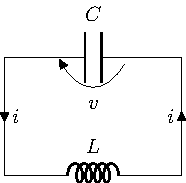
\includegraphics[width=0.4\linewidth]{sl_tsm/lckolo.pdf}
\caption{Резонантно коло.}
\label{tsm:fig:lckolo}
\end{figure}
Прво ће бити размотрено $LC$ колo као пример изолованог резонатора (сл.~\ref{tsm:fig:lckolo}). Напон и струја задовољавају диференцијалне једначине:
\begin{equation}
v = L \frac{d i}{d t}; \qquad i = -C \frac{d v}{d t}.
\end{equation}
Сменом се лако може добити једначина линеарног хармонијског осцилатора, са резонантном фреквенцијом $\omega_0 = \frac{1}{\sqrt{LC}}$. \emph{Амплитуда позитивне фреквенције} дефинише се као:
\begin{equation}
\alpha = \sqrt{\frac{C}{2}}\left( v + j\sqrt{\frac{L}{C}}i  \right),
\label{tsm:pamp}
\end{equation}
која задовољава диференцијалну једначину првог реда
\begin{equation}
\frac{d\alpha}{dt} = j\omega_0 \alpha.
\label{tsm:smdif1}
\end{equation}
Нормализација у \ref{tsm:pamp} је погодно одабрана тако да квадрат амплитуде $\alpha$ одговара снази:
\begin{equation}
|\alpha|^2 = \frac{C}{2}|V|^2 = W,
\end{equation}
док фаза одговара тренутној фази осцилација. За комплетан опис, потребно би било увести и променљиву, комплексно-конјуговану у односу на (\ref{tsm:pamp}), али показује се да је њу могуће занемарити. На овај начин је опис резонатора поједностављен.

\begin{figure}[h] 
\centering
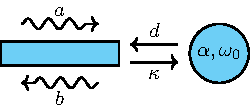
\includegraphics[width=0.4\linewidth]{sl_tsm/sm-vod1.pdf}
\caption{Спрега резонантног мода и вода.}
\label{tsm:fig:slike/smfig}
\end{figure}
Наравно, случај усамљеног резонатора није посебно занимљив; права вредност овог приступа се показује приликом разматрања спреге са водом. На сл.~ приказан је најједноставнији случај. У овом случају, јављају се два ефекта:
\begin{itemize}
\item енергија резонатора ,,цури`` у таласе на воду, што резонантни мод види као ефективне губитке;
\item инцидентни таласи врше побуду резонантног мода.
\end{itemize}
Најједноставнији пример шематски је приказан на сл.~\ref{tsm:fig:slike/smfig}, где је вод на свом крају спрегнут са резонантним модом. Поље на воду описано је таласним коефицијентима инцидентног, $a$, и рефлектованог таласа, $b$, према уобичајеној дефиницији за $S$-параметре. Математички, једначина (\ref{tsm:smdif1}) ће бити модификована на следећи начин
\begin{equation}
\frac{d\alpha}{dt} = j\omega_0 \alpha - \gamma \alpha + \kappa a,
\label{tsm:smdif2}
\end{equation}
где $\gamma$ представља коефицијент слабљења, а $\kappa$ коефицијент спреге инцидентног таласа и резонантног мода. За побуду константне фреквенције $\omega$, решење (\ref{tsm:smdif2}) гласи:
\begin{equation}
\alpha = \frac{\kappa a}{j(\omega-\omega_0) + \gamma}.
\label{tsm:haus:pobuda}
\end{equation}
С друге стране, рефлектовани талас на воду износиће
\begin{equation}
b = S_{11}^{(0)} a + d\alpha,
\label{tsm:haus:refl}
\end{equation}
где је $S_{11}^{(0)}$ коефицијент рефлексије у одсуству резонатора, а $d$ коефицијент спреге са рефлектованим таласом. Полазећи од закона одржања енергије, и симетрије Максвелових једначина у односу на измену знака времена, показује се да важи
\begin{equation}
\kappa = d,\qquad \gamma = \frac{1}{2}|d|^2.
\end{equation}
Комбиновањем (\ref{tsm:haus:pobuda}) и (\ref{tsm:haus:refl}) лако се добија израз за модификовани коефицијент рефлексије услед присуства резонатора:
\begin{equation}
S_{11} = \frac{b}{a} = S_{11}^{(0)} + \frac{d}{j(\omega-\omega_0) + {|d|^2}/{2}}.
\end{equation}

У случају два међусобно спрегнута резонатора, динамика система има следећи облик:
\begin{eqnarray}
\frac{d\alpha_1}{dt} & = j\omega_1 \alpha_1 + \kappa_{12} \alpha_2 , \\
\frac{d\alpha_2}{dt} & = j\omega_2 \alpha_2 + \kappa_{21} \alpha_1 , 
\label{tsm:haus:2sprenuta}
\end{eqnarray}
при чему због одржања енергије важи $\kappa_{12} = \kappa_{21}$.

Изразе (\ref{tsm:smdif1})--(\ref{tsm:haus:2sprenuta}) могуће је генералисати на случај $n$ (потенцијално спрегнутих) резонатора и $m$ улазно/излазних таласних портова
\begin{align}
\frac{\partial}{\partial t}
\begin{bmatrix}
\alpha_1 \\ \vdots \\ \alpha_n
\end{bmatrix}
& = \left(j\mathbf{\Omega} - \mathbf{\Gamma} \right)\begin{bmatrix}
\alpha_1 \\ \vdots \\ \alpha_n
\end{bmatrix}
+ \mathbf{D}^T
\begin{bmatrix}
a_1 \\ \cdots \\ a_m
\end{bmatrix}
\label{tsm:haus:evomat}\\
\intertext{за резонаторе, и}
\begin{bmatrix}
b_1 \\ \vdots \\ b_m
\end{bmatrix}
& = \mathbf{S}^{(0)}
\begin{bmatrix}
a_1 \\ \vdots \\ a_m
\end{bmatrix}
+\mathbf{D}\begin{bmatrix}
\alpha_1 \\ \vdots \\ \alpha_n
\end{bmatrix};
\label{tsm:haus:reflmat}
\end{align}
за рефлектоване таласе, где су
\begin{equation}
\mathbf{\Omega} = \begin{bmatrix}
\omega_1      & \cdots    & \kappa_{1n} \\
\vdots        & \ddots    & \vdots      \\
\kappa_{1n}^* & \cdots    & \omega_n    \\
\end{bmatrix}; \qquad
\mathbf{D} = \begin{bmatrix}
d_{11}  & \cdots  & d_{1m} \\
\vdots  & \ddots  & \vdots \\
d_{n1}  & \cdots  & d_{nm} \\
\end{bmatrix};\qquad \mathbf{\Gamma}=\frac{1}{2}\mathbf{D}^\dag \mathbf{D};
\label{tsm:haus:wdmat}
\end{equation}
а $\mathbf{S}^{(0)}$ представља ,,директну`` матрицу расејања, која карактерише систем у одсуству резонатора. Додатно, може се показати да важи следећа релација
\begin{equation}
\mathbf{S}^{(0)}\mathbf{D^*}=-\mathbf{D},
\label{tsm:haus:d_usl}
\end{equation}
помоћу које је могуће одредити фазе елемената матрице $\mathbf{D}$~\cite{wonjoo}.

%Изрази (\ref{tsm:cm_s21})--(\ref{tsm:cm_s11}) представљају рационалне функције. However, compared to the general methods~\cite{rationalfit}, CMT enables exploiting system geometry and significantly reducing the number of unknown parameters. Also, if field patterns of modes are known, CMT constants can be directly calculated~\cite{hausproc}.

\section{Примена? Резултати?}
\subsection{Антисиметрични сплит рингови}%

Микрострип водови, оптерећени са СРР резонаторима са варијабилним положајем процепа, приказани су на сл.~\ref{tsm:sl1a}-\ref{tsm:sl1}. У општем случају, постојаће спрега између два СРР-а, на основу чега се очекују две резонансе у спектру, услед цепања(?). Геометрије на сл.~\ref{tsm:sl1a} поседују рефлексиону симетрију у односу на раван, нормалну на супстрат, која садржи централну осу вода. Због ове симетрије, један мод не може бити побуђен, због чега ће бити присутна само једна резонанса у трансмисији~\cite{radoman}. С друге стране, геометрије на сл.~\ref{tsm:sl1}, које ћемо називати \emph{антисиметричним}, не поседују раван симетрије; уместо тога, симетричне су у односу на ротацију од \SI{180}{\degree} око централне тачке. У наставку ће ТСМ и анализа помоћу еквивалентне шеме бити примењена на структуре са сл.~\ref{tsm:sl1}.

Оно што антисиметричне структуре чини занимљивим јесте да испољавају мешовиту (електричну и магнетну) спрегу СРР-ова са водом, као и незанемарљиву спрегу између самих прстенова, а притом су електрично симетричне, због чега је могуће поједностављено их анализирати преко парне и непарне побуде. За разлику од структура са раванском симетријом, поседују две резонансе у трансмисионом спектру, које се могу независно подешавати. Са практичне тачке гледишта, ове структуре могу послужити као основа занимљивих ефеката, као што је класична аналогија ЕИТ-а~\cite{tassin:09,mr03:eit,cihan}. %These properties are suitable for various applications like slow light, delay lines and sensors.

\begin{figure}[!t]
\centering
\subfloat[]{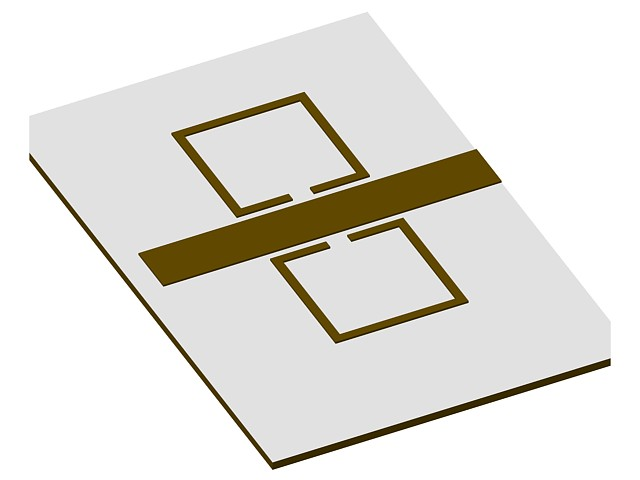
\includegraphics[width=0.42\columnwidth]{sl_tsm/pod0_1.jpeg}
\label{tsm:sl1:sim1}}%
\hfil
\subfloat[]{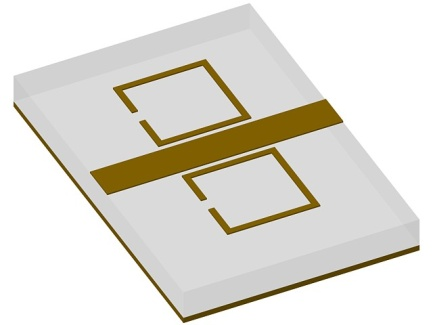
\includegraphics[width=0.42\columnwidth]{sl_tsm/pod90sim.jpeg}
\label{tsm:sl1:sim2}}\\
\subfloat[]{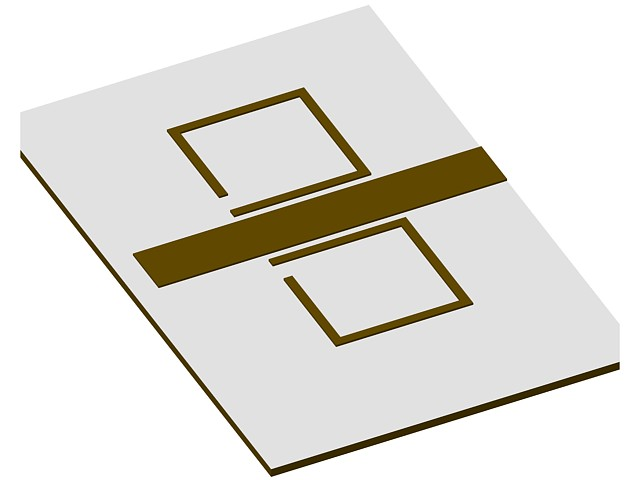
\includegraphics[width=0.42\columnwidth]{sl_tsm/pod90sim_cosak.jpeg}\label{tsm:sl1:sim3}}%
\hfil
\subfloat[]{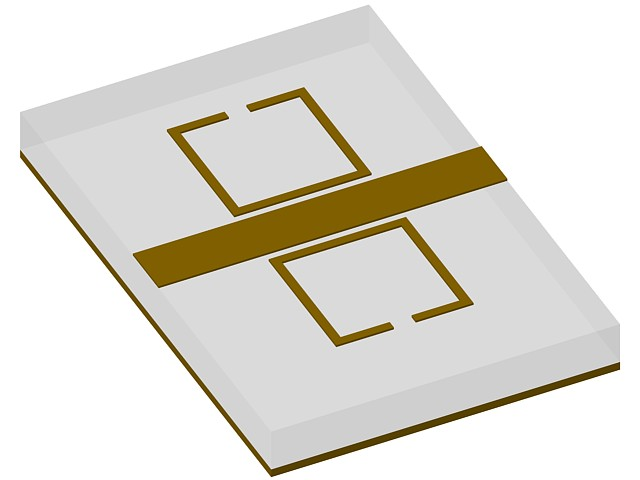
\includegraphics[width=0.42\columnwidth]{sl_tsm/pod180x2.jpeg}}
\caption{Микрострип вод спрегнут са два СРР-а у симетричној конфигурацији.}
\label{tsm:sl1a}
\end{figure}
\begin{figure}[!t]
\centering
\subfloat[]{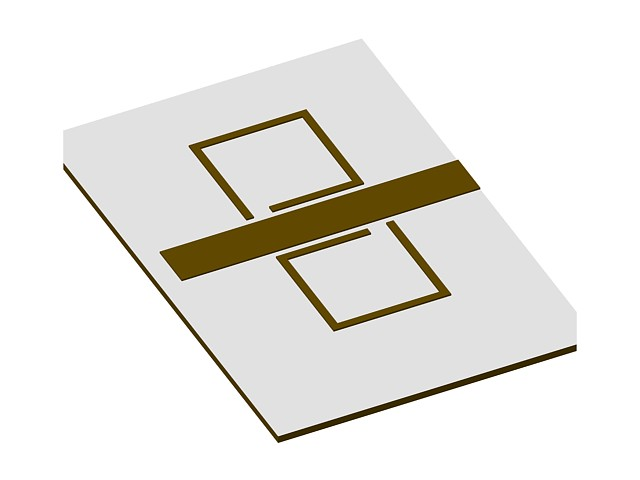
\includegraphics[width=0.48\columnwidth]{sl_tsm/pod0.jpeg}\label{tsm:sl1:pod0}}
\hfil
\subfloat[]{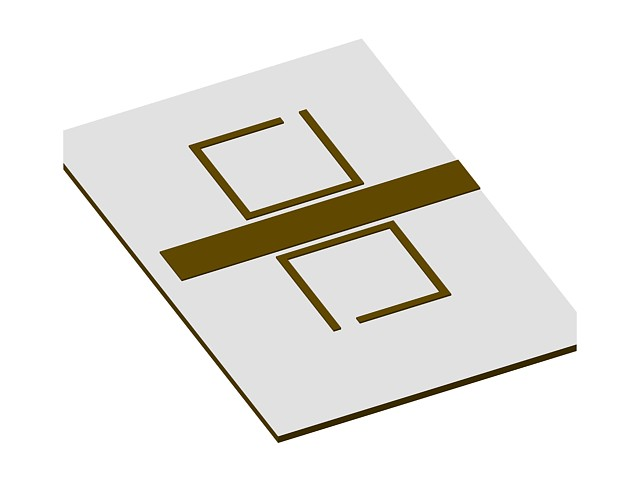
\includegraphics[width=0.48\columnwidth]{sl_tsm/pod180.jpeg}
\label{tsm:sl1:pod180}}\\
\subfloat[]{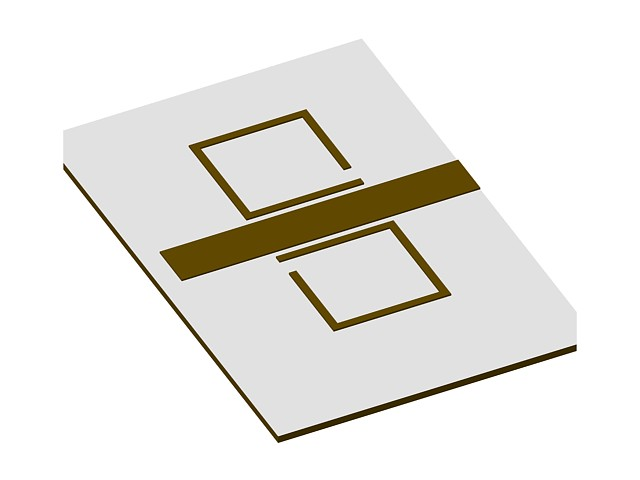
\includegraphics[width=0.48\columnwidth]{sl_tsm/pod90bg.jpeg}
\label{tsm:sl1:pod90bg}}%
\hfil
\subfloat[]{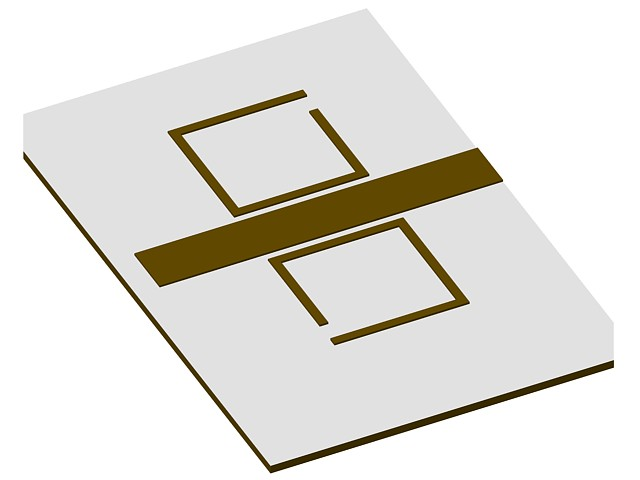
\includegraphics[width=0.42\columnwidth]{sl_tsm/pod90dv.jpeg}
\label{tsm:sl1:pod90dv}}\\
\subfloat[]{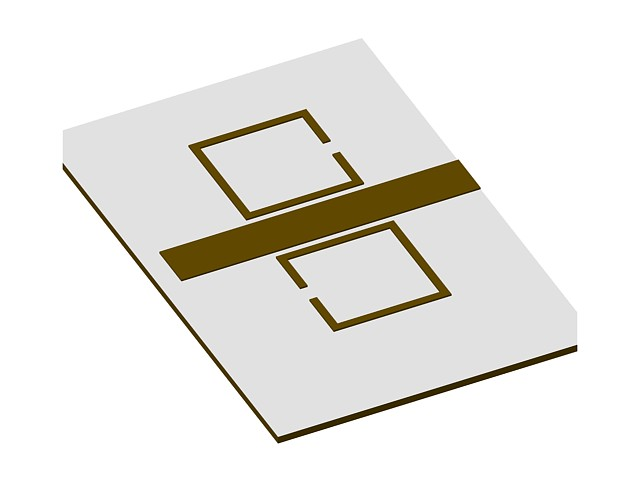
\includegraphics[width=0.48\columnwidth]{sl_tsm/pod90sr.jpeg}\label{tsm:sl1:pod90sr}}%
\caption{Микрострип вод спрегнут са два СРР-а у антисиметричној конфигурацији.}
\label{tsm:sl1}
\end{figure}

\subsection{Анализа помоћу ТСМ}\label{tsm:sec:cmt}
\begin{figure}
\centering
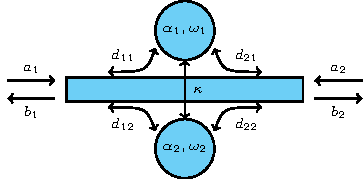
\includegraphics[scale=1]{sl_tsm/smfig.pdf}
\caption{Вод бочно спрегнут са два резонатора.}
\label{tsm:smfig}
\end{figure}

Шематски приказ геометрија са сл.~\ref{tsm:sl1a}--\ref{tsm:sl1}, у контексту ТСМ, дат је на сл.~\ref{tsm:smfig}. Систем се састоји од два резонатора и поседује два улазно/излазна порта, због чега димензије матрица $\mathbf{D}$, $\mathbf{S}$ и $\mathbf{\Omega}$, дефинисаних у (\ref{tsm:haus:wdmat}), износе $2\times 2$. Узимајући у обзир ротациону симетрију система, може се закључити да ове матрице имају следећи облик:
\begin{equation}
\mathbf{S}^{(0)} = \begin{bmatrix}
S^{(0)}_{11} & S^{(0)}_{21} \\
S^{(0)}_{21} & S^{(0)}_{11}
\end{bmatrix},\qquad
\mathbf{D} = \begin{bmatrix}
d_1 & d_2 \\
d_2 & d_1
\end{bmatrix},\qquad
\mathbf{\Omega} = \begin{bmatrix}
\omega_0 & -\kappa \\
-\kappa & \omega_0
\end{bmatrix},
\label{tsm:haus:sims}\end{equation}
при чему $\kappa\in \mathbb{R}$ у овом случају. У устаљеном режиму побуде, после замене (\ref{tsm:haus:evomat}) и (\ref{tsm:haus:sims}) у (\ref{tsm:haus:reflmat}), лако се добија решење за укупну трансмисију кроз систем:
\begin{equation}
\begin{split}
S_{21} = S^{(0)}_{21} + \frac{(d_1+d_2)^2}{2j(\omega-\omega_0 - \kappa) + |d_1+d_2|^2}\\
- \frac{(d_1-d_2)^2}{2j(\omega-\omega_0 + \kappa) + |d_1-d_2|^2},
\end{split}\label{tsm:cm_s21}
\end{equation}
и за рефлексију:
\begin{equation}
\begin{split}
S_{11} = S^{(0)}_{11} + \frac{(d_1+d_2)^2}{2j(\omega-\omega_0 - \kappa) + |d_1+d_2|^2}\\
+ \frac{(d_1-d_2)^2}{2j(\omega-\omega_0 + \kappa) + |d_1-d_2|^2}.
\end{split}\label{tsm:cm_s11}
\end{equation}
У изразима (\ref{tsm:cm_s21})-(\ref{tsm:cm_s11}), први разломак одговара парном (симетричном) а други немарном (антисиметричном) моду спрегнутих резонатора. Резонантне учестаности ових модова су $\omega_{\pm} = \omega_0 \pm \kappa$ и $Q$-фактори:
\begin{equation}
Q_\pm = \nicefrac{\omega_\pm}{\gamma_{\pm}},\qquad \gamma_{\pm} = |d_1 \pm d_2|^2
\end{equation}
где знак (+) одговара парном, а (-) непарном моду.
% * <vojislav_m@yahoo.com> 2017-11-01T16:59:28.761Z:
% 
% > where (+) sign corresponds to the even mode, and (-) to the odd mode.
% proveriiii!!!!
% 
% ^.

\subsection{Анализа помоћу еквивалентне шеме}\label{tsm:sec:eqcirc}
Еквивалентна шема за антисиметричну геометрију (сл.~\ref{tsm:sl1}) приказана је на сл.~\ref{tsm:sl3}. Укључује електричну и магнетну спрегу СРР-ова са водом, као и међусобну спрегу СРР-ова. Због једноставности, за анализу у овој секцији биће коришћена шена са једном П-ћелијом; приликом поређења резултата биће укључена и шема са две ћелије.

Шема са сл.~\ref{tsm:sl3} је електрично симетрична, због чега је погодно анализирати је преко парне/непарне побуде~\cite{hong}. Међутим, она не поседује рефлексиону симетрију, због чега није могуће одредити парне и непарне адмитансе на стандардни начин, постављањем електричног и магнетног зида у равни симетрије. Уместо тога, биће показано како се ротациона симетрија кола може искористити да се добију тражене адмитансе.

На почетку приметимо да сви одзиви у колу представљају билинеарне функције улазних параметара, нпр.
\begin{equation}
I_{S1} = \mathcal{L}_{I_{S1}}(V_1,V_2) = -\mathcal{L}_{I_{S1}}(-V_1,-V_2).
\label{tsm:blin1}\end{equation}
Услед антисиметрије, следећа релација мора важити (за референтне смерове са сл.~\ref{tsm:sl3}):
\begin{equation}
    I_{S2}=\mathcal{L}_{I_{S2}}(V_1,V_2)=\mathcal{L}_{I_{S1}}(V_2,V_1).
\label{tsm:blin2}\end{equation}
\begin{table}[!t]
\renewcommand{\arraystretch}{1.3}
\caption{Одзиви у еквивалентном колу за парну и непарну побуду.}
\label{tsm:tabela_uslovi}
\centering
\begin{tabular}{|c|c|}
\hline
парна & непарна \\
\hline
$V_1 = V_2$ & $V_1 = -V_2$ \\
\hline
$I_{S1} = I_{S2}$ & $I_{S1} = -I_{S2}$ \\
\hline
$V_{S1} = V_{S2}$ & $V_{S1} = -V_{S2}$ \\
\hline
$I_L = 0$ & $I_L$ произвољно\\
\hline
\end{tabular}
\end{table}
\begin{figure}
    \begin{center}
        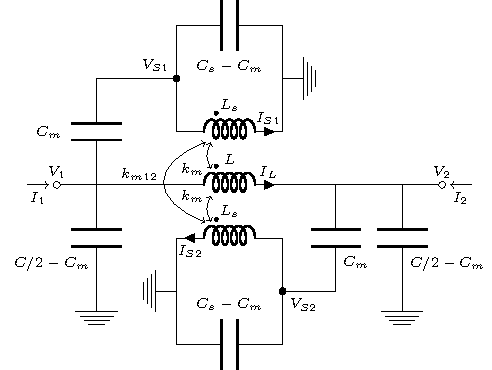
\includegraphics[scale=1]{sl_tsm/sl3.pdf}
    \caption{Еквивалентна шема за структуре са сл.~\ref{tsm:sl1}.}
    \label{tsm:sl3}
  \end{center}
\end{figure}
\begin{figure}[!t]
\centering
\subfloat[]{
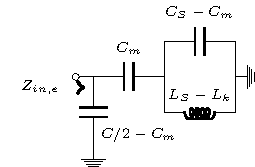
\includegraphics[scale=1.3]{sl_tsm/ekv_par.pdf}\label{tsm:ekv_par}}
\hfil
\subfloat[]{
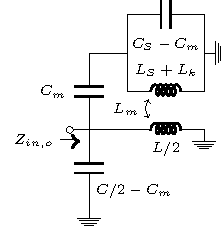
\includegraphics[scale=1.3]{sl_tsm/ekv_nepar.pdf}\label{tsm:ekv_nepar}}
\caption{Еквивалентна шема за (а) парну и (б) непарну побуду ($L_k=k_{m12}L_S$).}
\label{tsm:sl4}
\end{figure}
Коришћењем (\ref{tsm:blin1}) и (\ref{tsm:blin2}), могуће је одредити релације за одзиве у колу, при парној и непарној побуди, и оне су сумиране у табели~\ref{tsm:tabela_uslovi}. На основу тога, могуће је одредити поједностављена кола за парну и непарну екситацију, која су приказана на сл.~\ref{tsm:sl4}. На основу њих можемо израчунати парну и непарну адмитансу, $y_{e,o}$, нормализовану на $Y_0=\sqrt{C/L}$
%\begin{equation}
%\begin{aligned}
%Y_e &=j\omega\frac{C}{2}\left(1-2k_e^2+\chi\right); \\
%Y_o &=j\omega\frac{C}{2}\left(1-2k_e^2\right) - \frac{2j}{\omega L}\xi;\\
%\chi &=\frac{2k_e^2}{1-\omega ^2 C_S L_S(1-k_{m12})}; \\
%\xi &= \frac{1 - \omega ^2 \left( C_S L_S(1+k_{m12})-2C_m L_m+k_e^2 \frac{LC}{2}\right)}{1-\omega^2C_S L_S \left(1+k_{m12}-2k_m^2\right)}.
%\end{aligned}
%\end{equation}
\begin{equation}
\begin{aligned}
y_e &= y_e^\Pi + \frac{j}{2}\frac{\omega}{\omega_{LC}}\frac{2\gamma_e^2}{1-\omega^2 / \omega_e^2}, \\
y_e^\Pi &= \frac{j}{2}\frac{\omega}{\omega_{LC}}\left(1 - 2 k_e^2\right), \\
y_o &=  y_o^\Pi + \frac{j}{2}\frac{\omega}{\omega_{LC}}\frac{2\gamma_o^2}{1-\omega^2 / \omega_o^2}, \\
y_o^\Pi &= \frac{j}{2}\frac{\omega}{\omega_{LC}}\left(1 - 2 k_e^2\right) - 2j\frac{\omega_{LC}}{\omega}
;
\end{aligned}
\label{tsm:eo}
\end{equation}
где је
\begin{equation}
\begin{aligned}
\gamma_e &= k_e, \\
\gamma_o &= 2\omega_{LC}\sqrt{L_S C_S} k_m - k_e, \\
\omega_e &= 1/ \sqrt{L_S C_S(1-k_{m12})}, \\
\omega_o &= 1/ \sqrt{L_S C_S(1+k_{m12}-2k_m^2)}, \\
\omega_{LC} &= 1/ \sqrt{LC}.
\end{aligned}
\label{tsm:eo_pom}
\end{equation}
У (\ref{tsm:eo}) раздвојени су нерезонантни делови адмитанси преко чланова $y_{e,o}^\Pi$. Они представљају парну  и непарну адмитансу само П-ћелије на.~\ref{tsm:sl3}, односно потичу само од вода.\footnote{Треба приметити да су $y_{e,o}^\Pi$ пертурбовани у односу на изоловани вод, услед присуства СРР-ова, али овај ефекат је врло мали.} Ова нотација ће олакшати поређење са резултатима ТСМ, као што ће се видети касније. Према~\cite{hong}, коефицијент трансмисије, $S_{21}$, износи:
\begin{equation}
\begin{aligned}
S_{21} =& \frac{1}{2}(S_{11,e}-S_{11,o}) \\
=& \frac{1}{2}\left( \frac{1-y_e}{1+y_e}
- \frac{1-y_o}{1+y_o} \right).
\end{aligned}
\end{equation}
Нерезонантни део трансмисије може се изразити преко чланова $y_{e,o}^\Pi$ (\ref{tsm:eo}):
\begin{equation}
S_{21}^\Pi = \frac{1}{2} \left( S_{11e}^\Pi - S_{11o}^\Pi \right),\quad
S_{11e,o}^\Pi = \frac{1-y_{e,o}^\Pi}{1+y_{e,o}^\Pi},
\label{tsm:spi}\end{equation}
Што је еквивалентно матрици ,,директног`` расејања $\mathbf{S}^{(0)}$ из секције~\ref{tsm:sec:cmt}. Заменом (\ref{tsm:eo}), (\ref{tsm:eo_pom}) и (\ref{tsm:spi}), после сређивања, добија се коначни израз за трансмисију:
\begin{equation}
S_{21} = S_{21}^\Pi - \frac{S_{11,e}^\Pi\gamma'_e}{j(\omega^2-\varpi_e^2)+\gamma'_e} + \frac{S_{11,o}^\Pi\gamma'_o}{j(\omega^2-\varpi_o^2)+\gamma'_o},
\label{tsm:s21sm}\end{equation}
где је
\begin{equation}
\gamma'_{e,o} = \operatorname{Re}\left\{ \frac{1}{1+y_{e,o}^\Pi} \right\} \frac{\omega}{\omega_{LC}}\omega_{e,o}^2\gamma_{e,o}^2,
\label{tsm:gama}\end{equation}
\begin{equation}
\varpi_{e,o} = \omega_{e,o} - \operatorname{Im}\left\{ \frac{1}{1+y_{e,o}^\Pi} \right\} \frac{\omega}{\omega_{LC}}\omega_{e,o}^2\gamma_{e,o}^2.
\label{tsm:omega}\end{equation}
Облик (\ref{tsm:s21sm}) је намерно изабран како би се нагласила аналогија са резултатом ТСМ (\ref{tsm:cm_s21}). Важна разлика је да, уместо константних вредности за ТСМ, у (\ref{tsm:s21sm}) имамо функције учестаности, дефинисане са (\ref{tsm:gama})-(\ref{tsm:omega}). Ипак, ове функције споро варирају у поређењу са резонантним члановима, због чега су оба израза приближно еквивалентна у околини резонанси. У табели~\ref{tsm:tabela_ekv} приказано су релације које повезују параметре кола са константама за ТСМ, које се могу одредити на овај начин фиксирањем $\omega$ на жељеној фреквенцији.
\begin{table}[!t]
\renewcommand{\arraystretch}{2.8}
\caption{Релације између константи за ТСМ и параметара кола.}
\label{tsm:tabela_ekv}
\centering
\begin{tabular}{|c|c|}
\hline
ТСМ & Еквивалентна шема \\
\hline
$\omega_+$ & $\omega_{e} - \operatorname{Im}\left\{ \frac{1}{1+y_{e}^\Pi} \right\} \frac{\omega\omega_{e}^2}{\omega_{LC}(\omega + \omega_e)}\gamma_{e}^2$ \\
\hline
$\omega_-$ & $\omega_{o} - \operatorname{Im}\left\{ \frac{1}{1+y_{o}^\Pi} \right\} \frac{\omega\omega_{o}^2}{\omega_{LC}(\omega + \omega_o)}\gamma_{o}^2$ \\
\hline
$\gamma_+$ & $\operatorname{Re}\left\{ \frac{1}{1+y_{e}^\Pi} \right\} \frac{2\omega\omega_{e}^2}{\omega_{LC}(\omega + \omega_e)}\gamma_{e}^2$ \\
\hline
$\gamma_-$ & $\operatorname{Re}\left\{ \frac{1}{1+y_{o}^\Pi} \right\} \frac{2\omega\omega_{o}^2}{\omega_{LC}(\omega + \omega_o)}\gamma_{o}^2$\\
\hline
\end{tabular}
\end{table}

Фреквенцијска зависност ефективних резонантних фреквенција модова $\varpi_{e,o}$ и јачина спреге $\gamma'_{e,o}$ у (\ref{tsm:s21sm})--(\ref{tsm:omega}) може бити образложена на следећи начин. П-ћелија која у колу представља вод се такође понаша као резонатор, додуше са знатно вишом резонантном фреквенцијом од СРР-ова. Ипак, спрега са водом узрокује фреквенцијски зависну пертурбацију, евидентну у (\ref{tsm:gama})--(\ref{tsm:omega}). Како би се добили аналитички изрази за параметре расејања, који су довољно једноставни да би били практично употребљиви, обично је неопходно занемарити овакве пертурбације. Међутим, ово није лак задатак полазећи од Кирхофових закона за еквивалентно коло, пошто је тешко унапред знати шта се може занемарити, а шта не. Насупрот томе, ТСМ даје изразе као што су (\ref{tsm:cm_s21}) директно, зато што инхерентно раздваја трансмисиони медијум и резонаторе, осим спреге првог реда. Због тога, она представља природни алат за анализу расејања у системима спрегнутих резонатора.

\section{Резултати и поређење}\label{tsm:sec:res}
\subsection{Валидација аналогије између два модела}
\begin{figure}[!t]
\centering
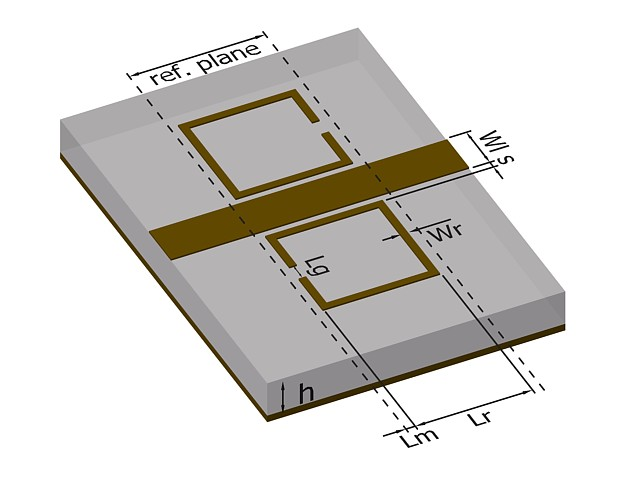
\includegraphics[width=7cm]{sl_tsm/dim3.jpeg}
\caption{Релевантне димензије:  $h = \SI{1.27}{\mm}$, $L_r = \SI{3}{\mm}$, $L_m = \SI{0.25}{\mm}$, $L_g = \SI{0.5}{\mm}$, $W_r = \SI{0.2}{\mm}$, $W_l = \SI{1.2}{\mm}$ и $s = \SI{0.1}{\mm}$.}
\label{tsm:dim}
\end{figure}
\begin{figure}
    \begin{center}
        \subfloat[]{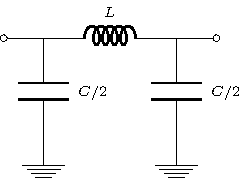
\includegraphics[scale=0.7]{sl_tsm/vod1cel.pdf}\label{tsm:slvod:1cel}}\hfil
        \subfloat[]{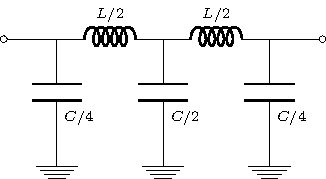
\includegraphics[scale=0.7]{sl_tsm/vod2cel.pdf}\label{tsm:slvod:2cel}}	
    \caption{Еквивалентна шема вода са: (а) једном, и (б) две П-ћелије.}
    \label{tsm:sl:vod2cel}
  \end{center}
\end{figure}
\begin{figure}[!t]
\centering
\subfloat[]{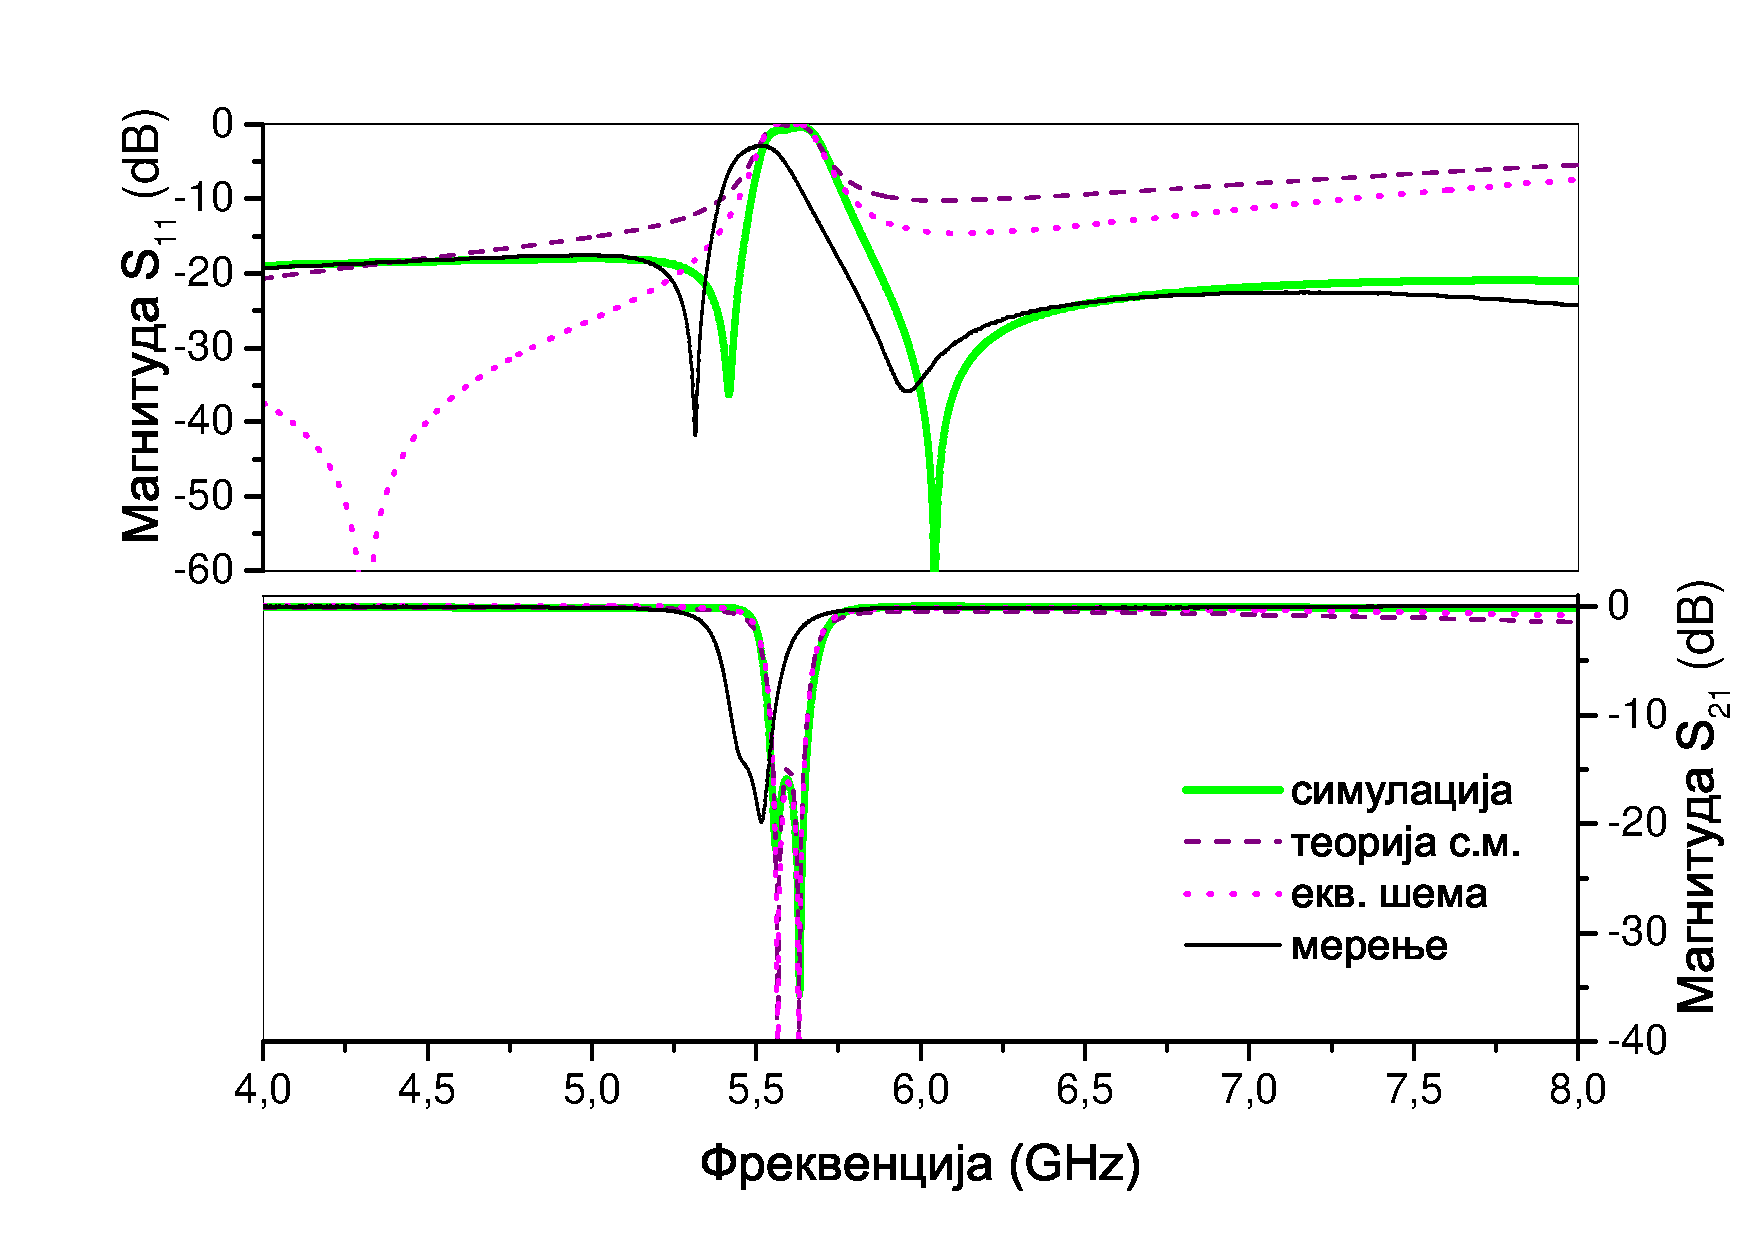
\includegraphics[width=0.5\textwidth]{sl_tsm/pod0/c2_mag.pdf}}\\
\subfloat[]{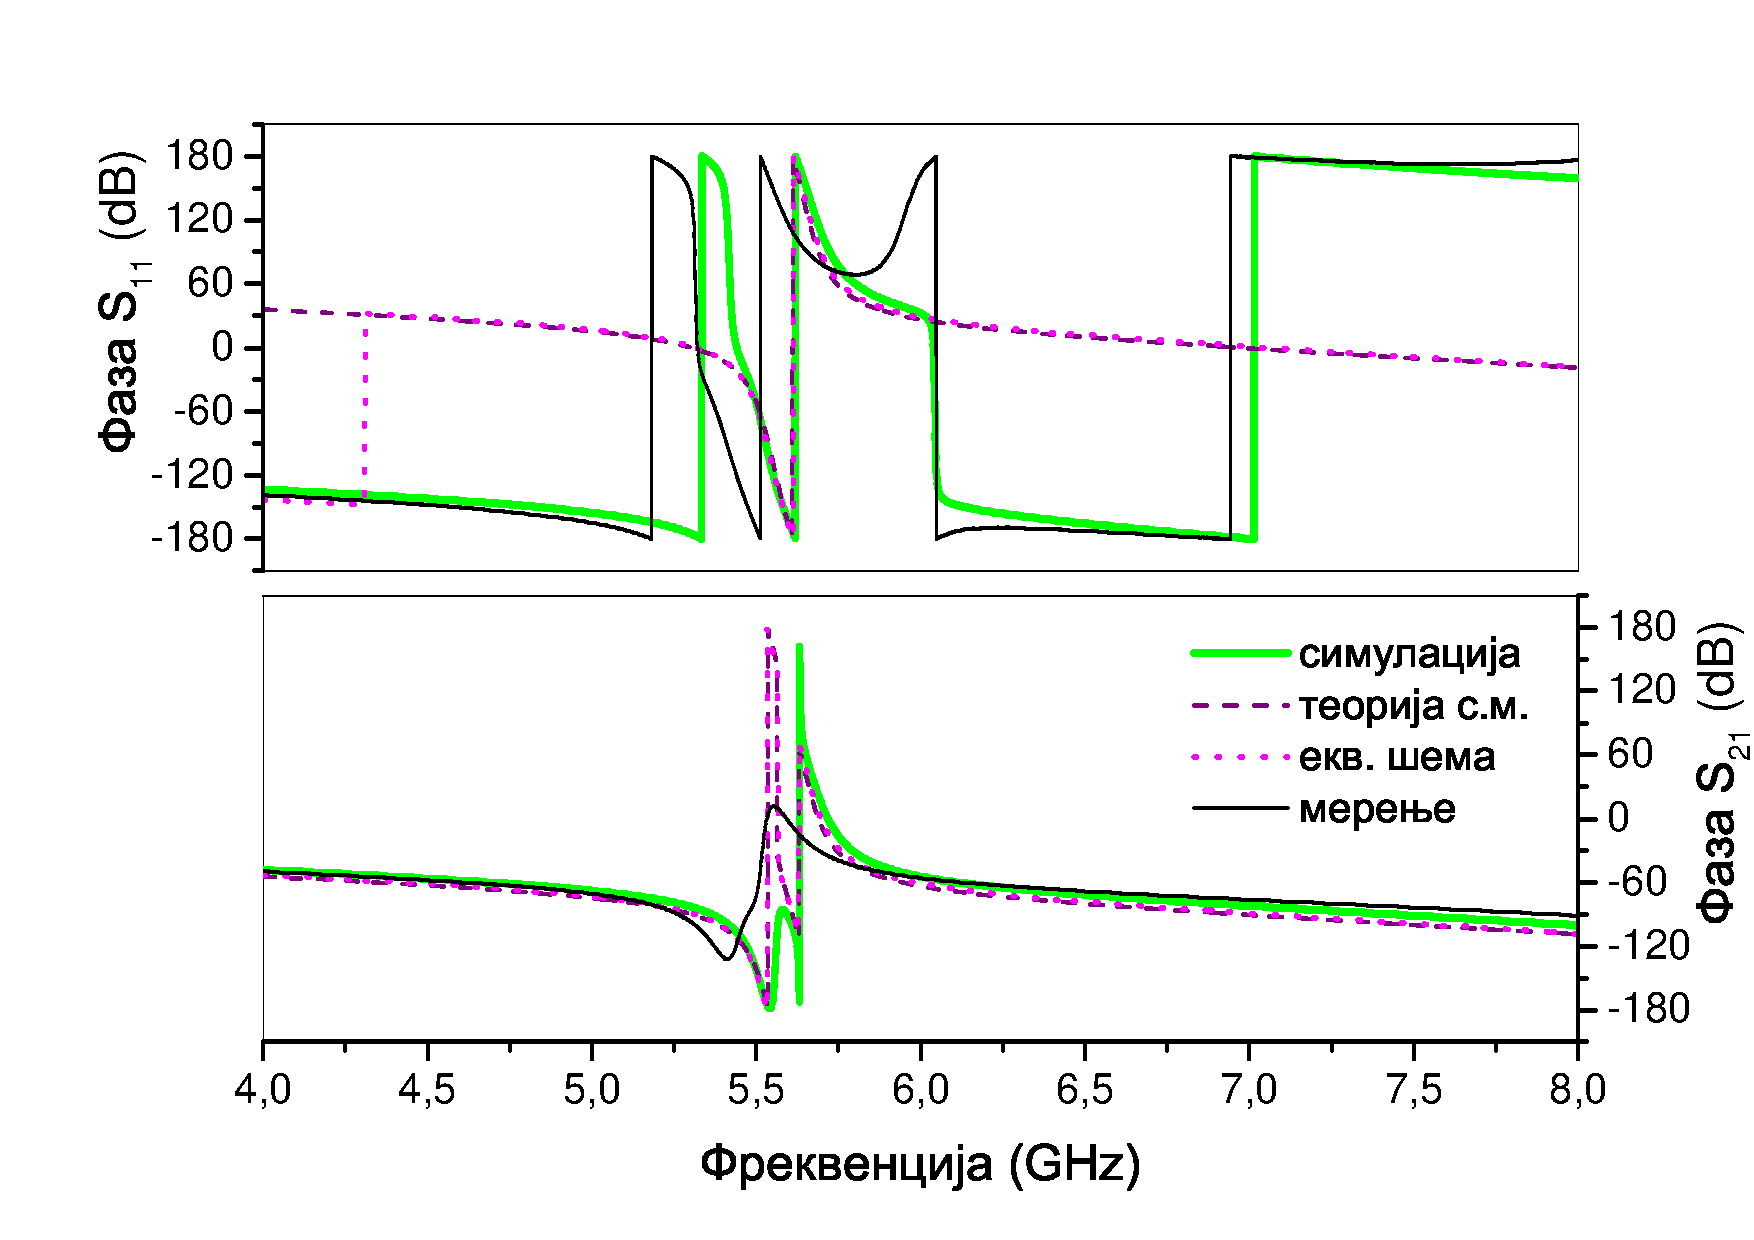
\includegraphics[width=0.5\textwidth]{sl_tsm/pod0/c2_faza.pdf}}
\caption{Магнитуда и фаза $S$-параметара за модел са сл.~\ref{tsm:sl1:pod0}}
\label{tsm:rez1c:pod0}
\end{figure}
\begin{figure}[!t]
\centering
\subfloat[]{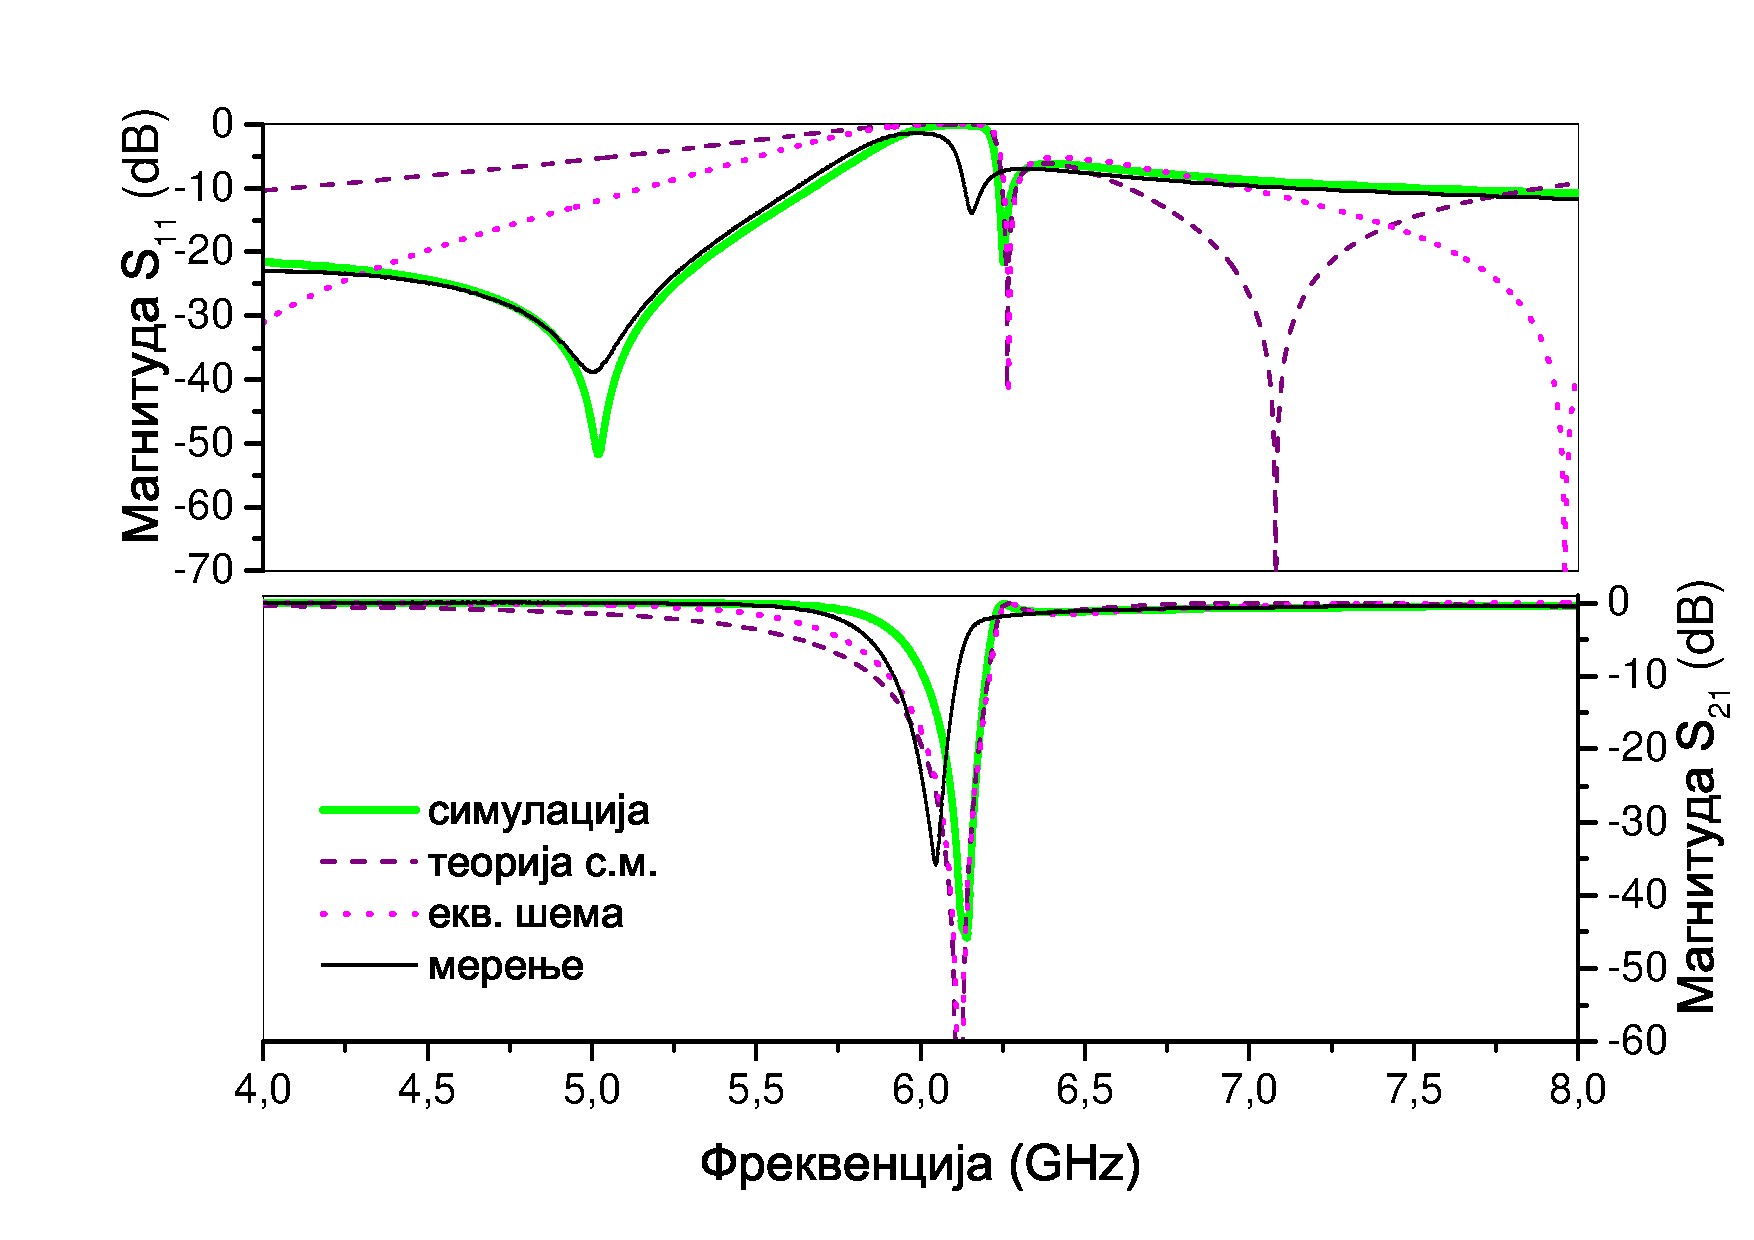
\includegraphics[width=0.5\textwidth]{sl_tsm/pod180/c2_mag.pdf}}\\
\subfloat[]{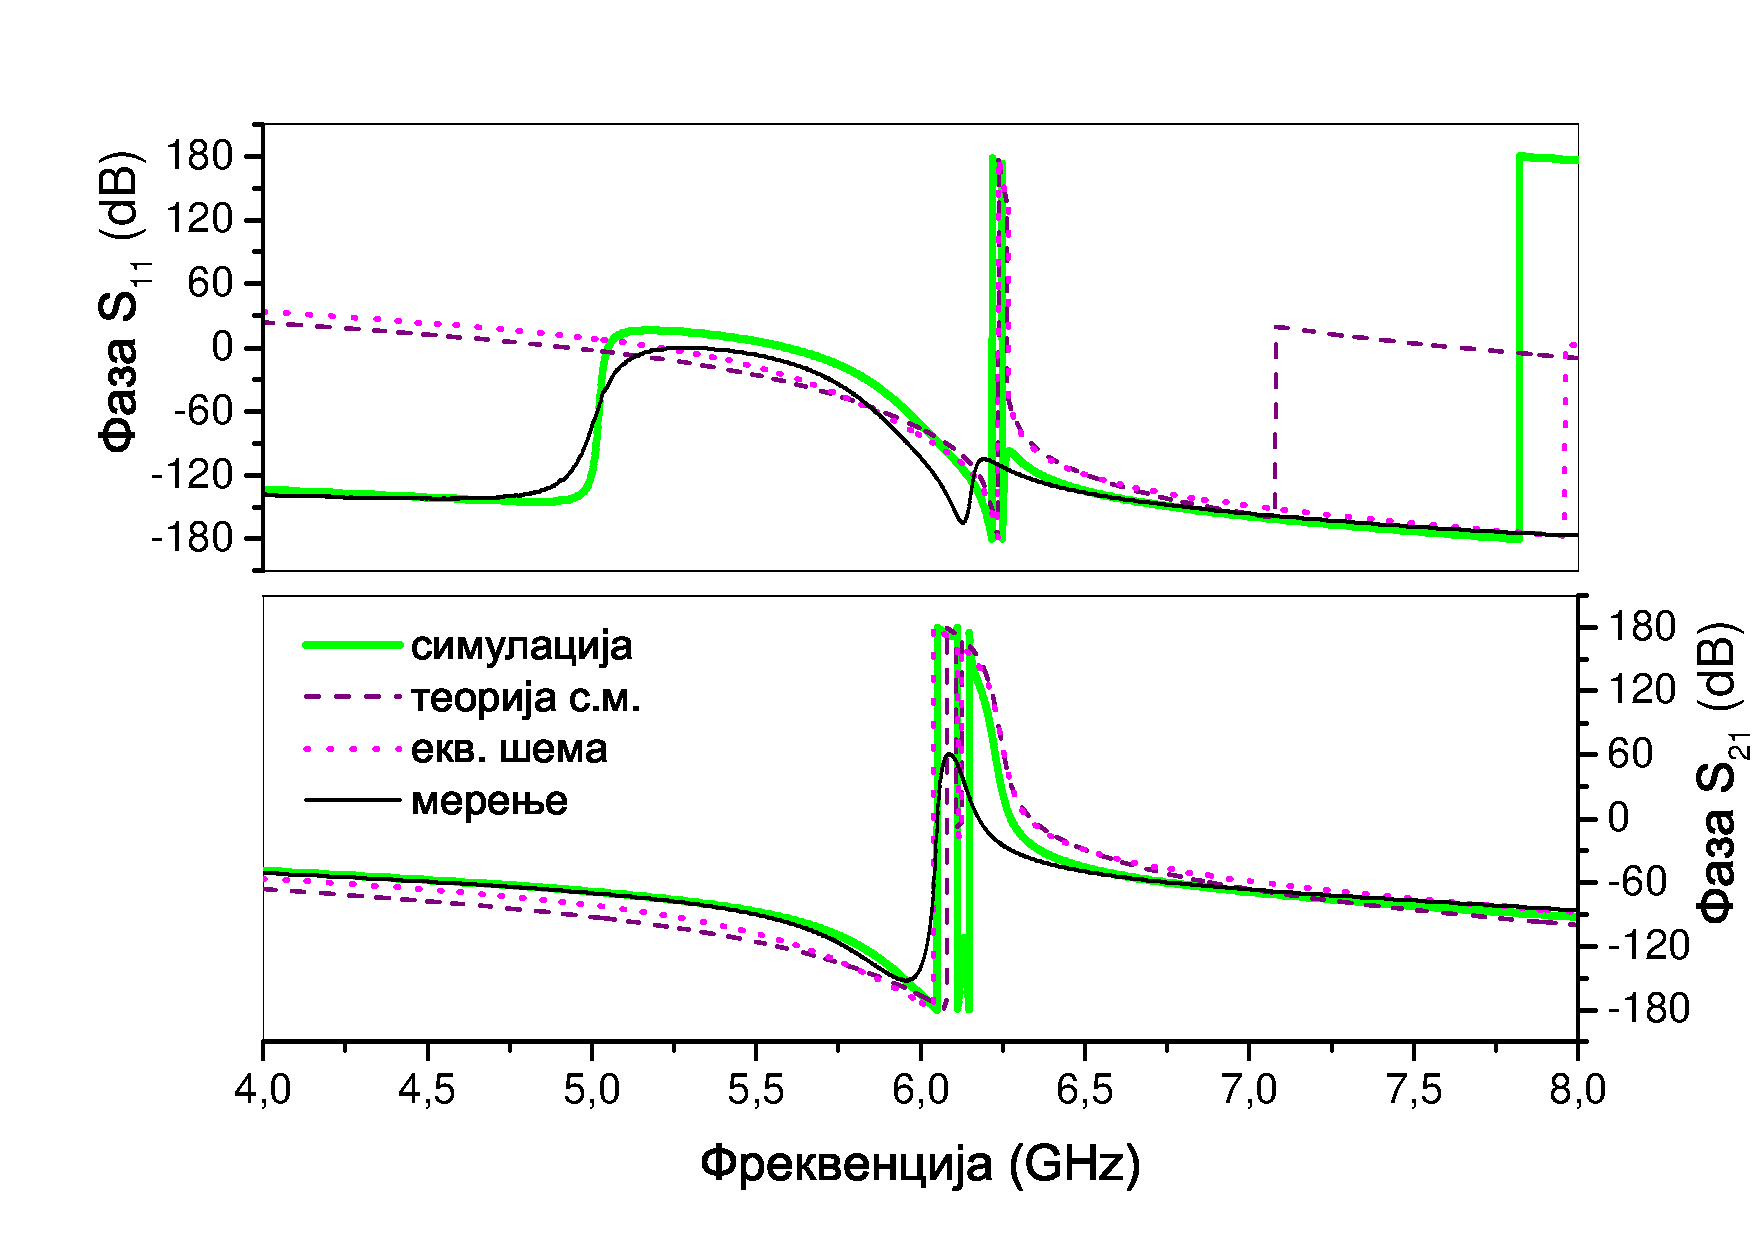
\includegraphics[width=0.5\textwidth]{sl_tsm/pod180/c2_faza.pdf}}
\caption{Магнитуда и фаза $S$-параметара за модел са сл.~\ref{tsm:sl1:pod180}}
\label{tsm:rez1c:pod180}
\end{figure}
Како би се тестирали предложени модели и упоредили њихови резултати, извршена је 3Д електромагнетна симулација структура са сл.~\ref{tsm:sl1}, док су \subref{tsm:sl1:pod0}, \subref{tsm:sl1:pod180}, \subref{tsm:sl1:pod90bg} и \subref{tsm:sl1:pod90sr} такође фабриковани и измерени. Релевантне димензије дате су на сл.~\ref{tsm:dim}, а коришћени диелектрични супстрат је Rogers RO3010 са $\varepsilon_r = \num{10.2}$. 

Најпре су одређени параметри еквивалентног кола. Како би се добили $L$, $C$ и $L_S$, микрострип вод и две најближе гране СРР-а су моделовани као секција вишепроводничког вода. Програм LINPAR~\cite{djordjevic1999linpar} је коришћен за нумерички прорачун квази-статичких параметара. На овај начин се добијају подужне капацитивности и индуктивности, из којих се тражене вредности $L$, $C$ и $L_S$ добијају множењем са одговарајућим дужинама~\cite{radoman}. Преостали параметри се добијају фитовањем кривих на резултате симулација.

Нелдер--Мидова симплекс метода~\cite{simplex} је коришћена за фитовање, са функцијом грешке која интеграли апсолутну разлику ($L^1$ норму) између симулираних података и параметризованог модела, у спектру од \SI{4}{\giga\hertz} до \SI{8}{\giga\hertz}:
\begin{equation}
\mathrm{Err}=\int_{f_\mathrm{min}}^{f_\mathrm{max}}\sum_{i=1}^2\sum_{j=1}^2\ \left | S_{ij}^\mathrm{model} - S_{ij}^{\mathrm{sim}} \right | df.
\end{equation}
У неким случајевима, тежинска функција је ручно повећавана у околини резонанси, како би више одговарала ускопојасној природи апроксимације. Иста процедура је коришћена у свим осталим случајевима фитовања у овој глави.

%the first question is how to generate non-resonant parameters $\mathbf{S}^{(0)}$ required in expressions (\ref{tsm:cm_s21})-(\ref{tsm:cm_s11}). Simplest approach would be to take them as constants; however, in order to make the best possible comparison with equivalent circuit analysis, we decided to use network of two $\Pi$ cells representing the transmission line (Fig.~\ref{tsm:sl:vod2cel}). In this approach, both models have essentially the same non-resonant parts, and the difference comes from the way resonators are included.
Константе за ТСМ добијене су коришћењем израза на десној страни табеле~\ref{tsm:tabela_ekv}, који су израчунати на фреквенцији између резонанси. Преостаје да се одреди матрица директног расејања $\mathbf{S}^{(0)}$, што се може извести на више начина. На пример, могле би се користити константе које би се фитовале, или би се ова матрица могла добити на основу симулације секције изолованог вода. У овом случају, $\mathbf{S}^{(0)}$ је прорачуната на основу електричне шеме кола које се састоји само од једне П-ћелије (сл.~\ref{tsm:slvod:1cel}), са истим вредностима $L$ и $C$ као у еквивалентном колу. Ово омогућава најприближније поређење два модела.

Резултати за две структуре са.~\ref{tsm:sl1} су приказани на сл.~\ref{tsm:rez1c:pod0}-\ref{tsm:rez1c:pod180}. Може се видети да се еквивалентна шема и ТСМ скоро у потпуности поклапају око резонанси, док постоје одступања у ширем опсегу, у складу са закључцима из секције~\ref{tsm:sec:eqcirc}. Надаље, оба метода показују добро поклапање са симулацијама у магнитуди и фази трансмисије ($S_{21}$ параметар) у целом опсегу; с друге стране, у случају рефлексије ($S_{11}$ параметар), добро поклапање постоји само у околини резонанси.

\subsection{Побољшани резултати}
\begin{figure}
    \begin{center}
        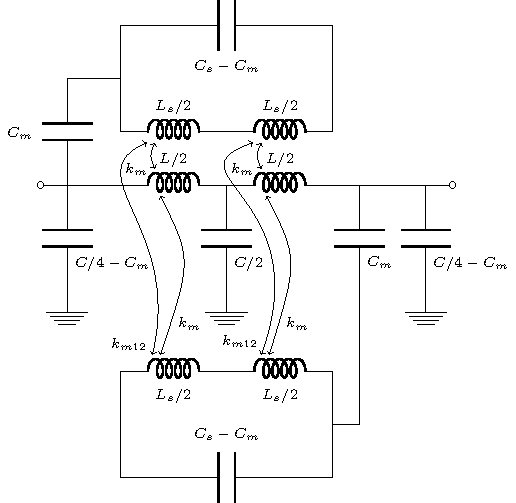
\includegraphics[scale=1]{sl_tsm/ekv2cel.pdf}
    \caption{Еквивалентна шема за антисиметричне структуре са две П-ћелије.}
    \label{tsm:sl:ekv2cel}
  \end{center}
\end{figure}
\begin{figure}[!t]
\centering
\subfloat[]{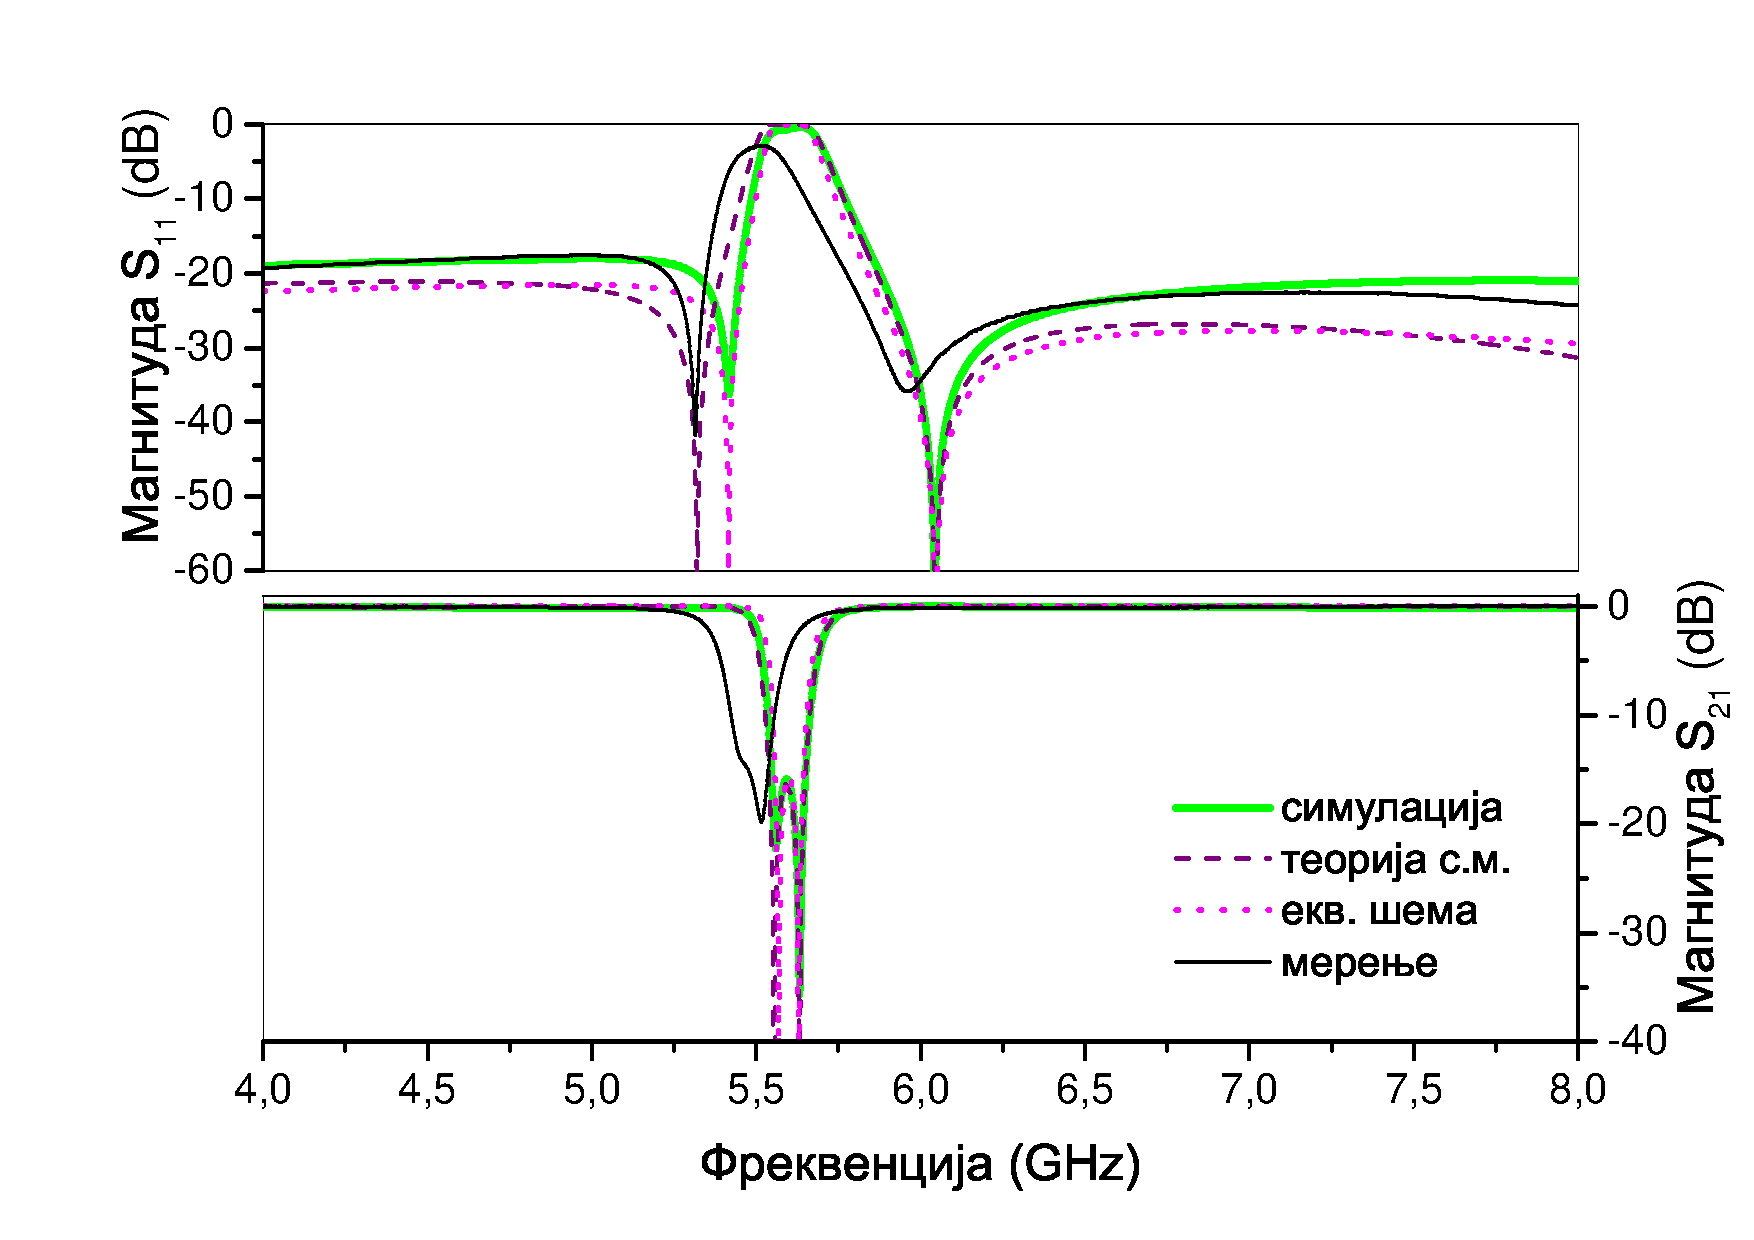
\includegraphics[width=0.5\textwidth]{sl_tsm/pod0/c_mag.pdf}}\\
\subfloat[]{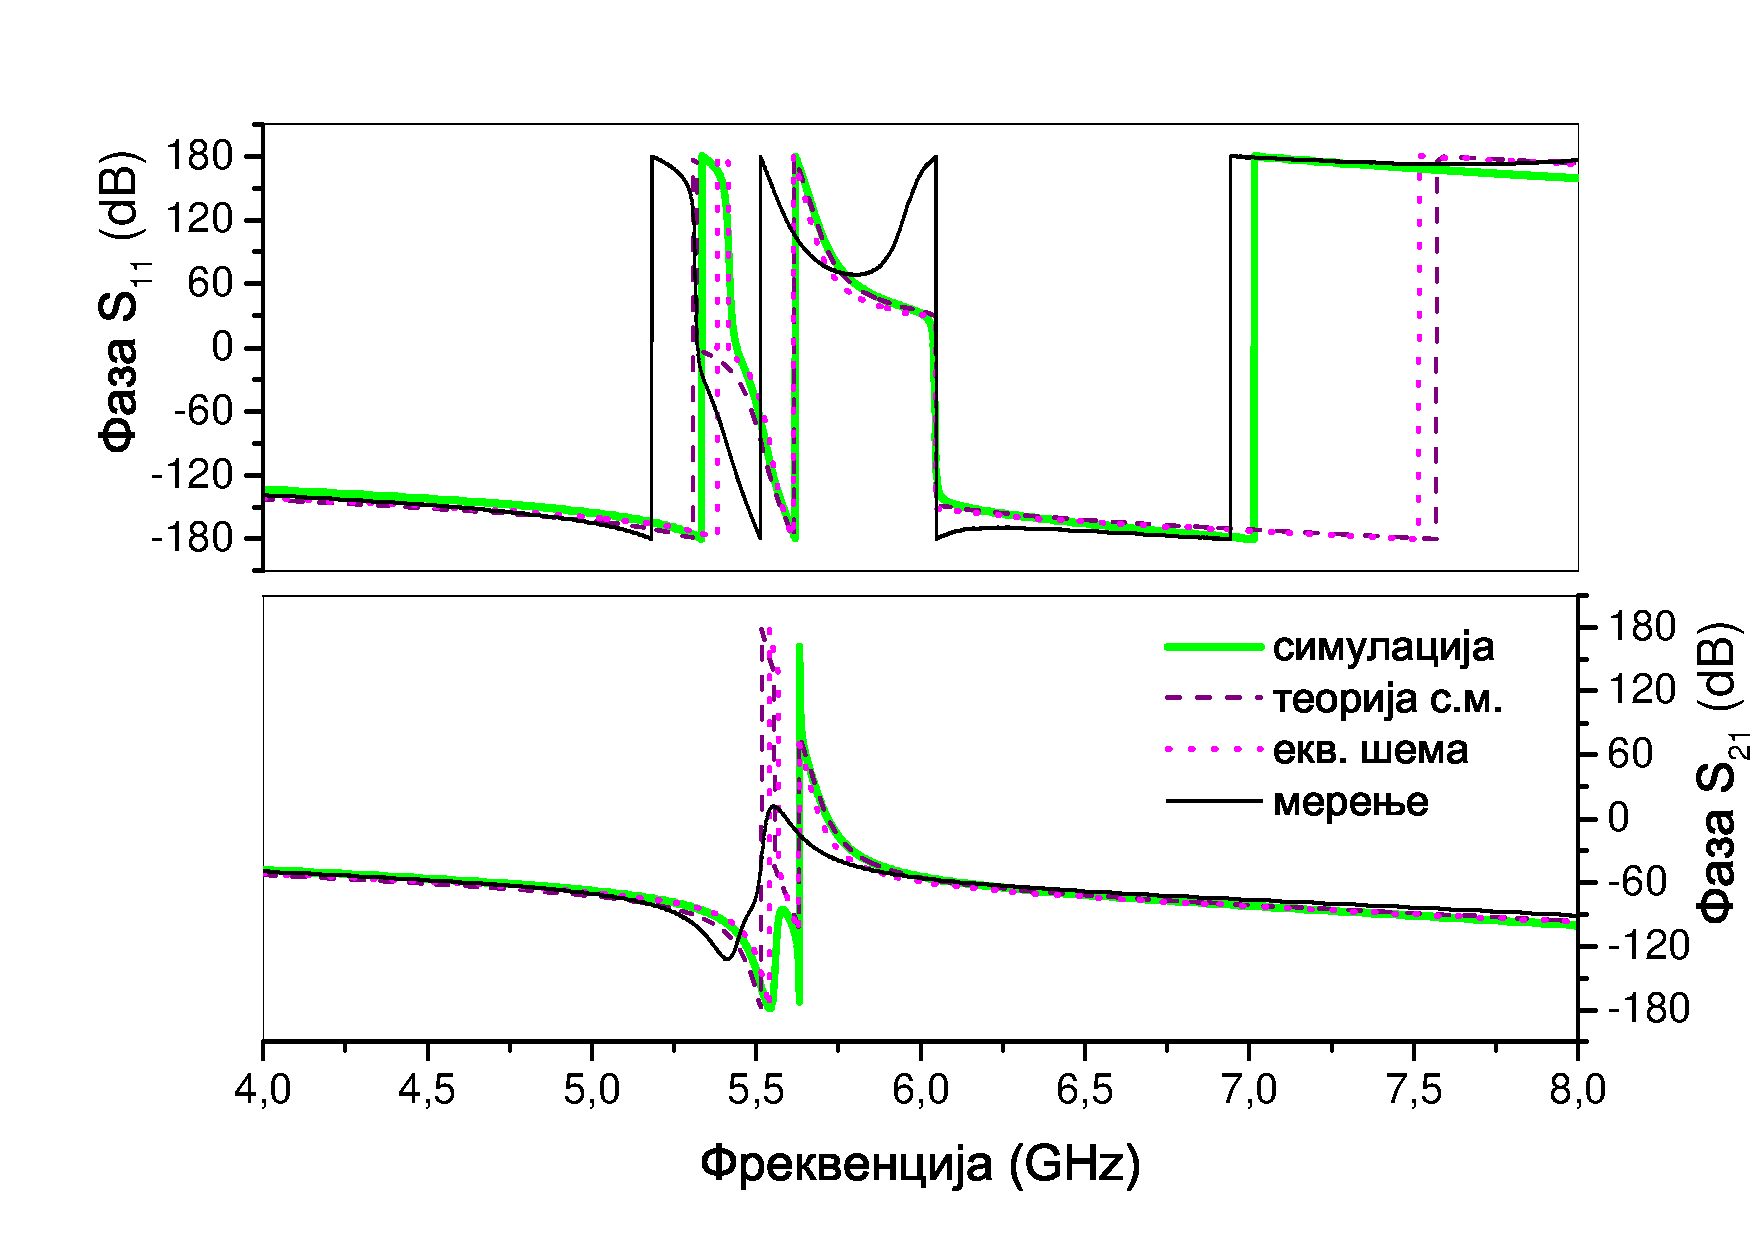
\includegraphics[width=0.5\textwidth]{sl_tsm/pod0/c_faza.pdf}}
\caption{Магнитуда и фаза $S$-параметара за модел са сл.~\ref{tsm:sl1:pod0}}
\label{tsm:rez:pod0}
\end{figure}
\begin{figure}[!t]
\centering
\subfloat[]{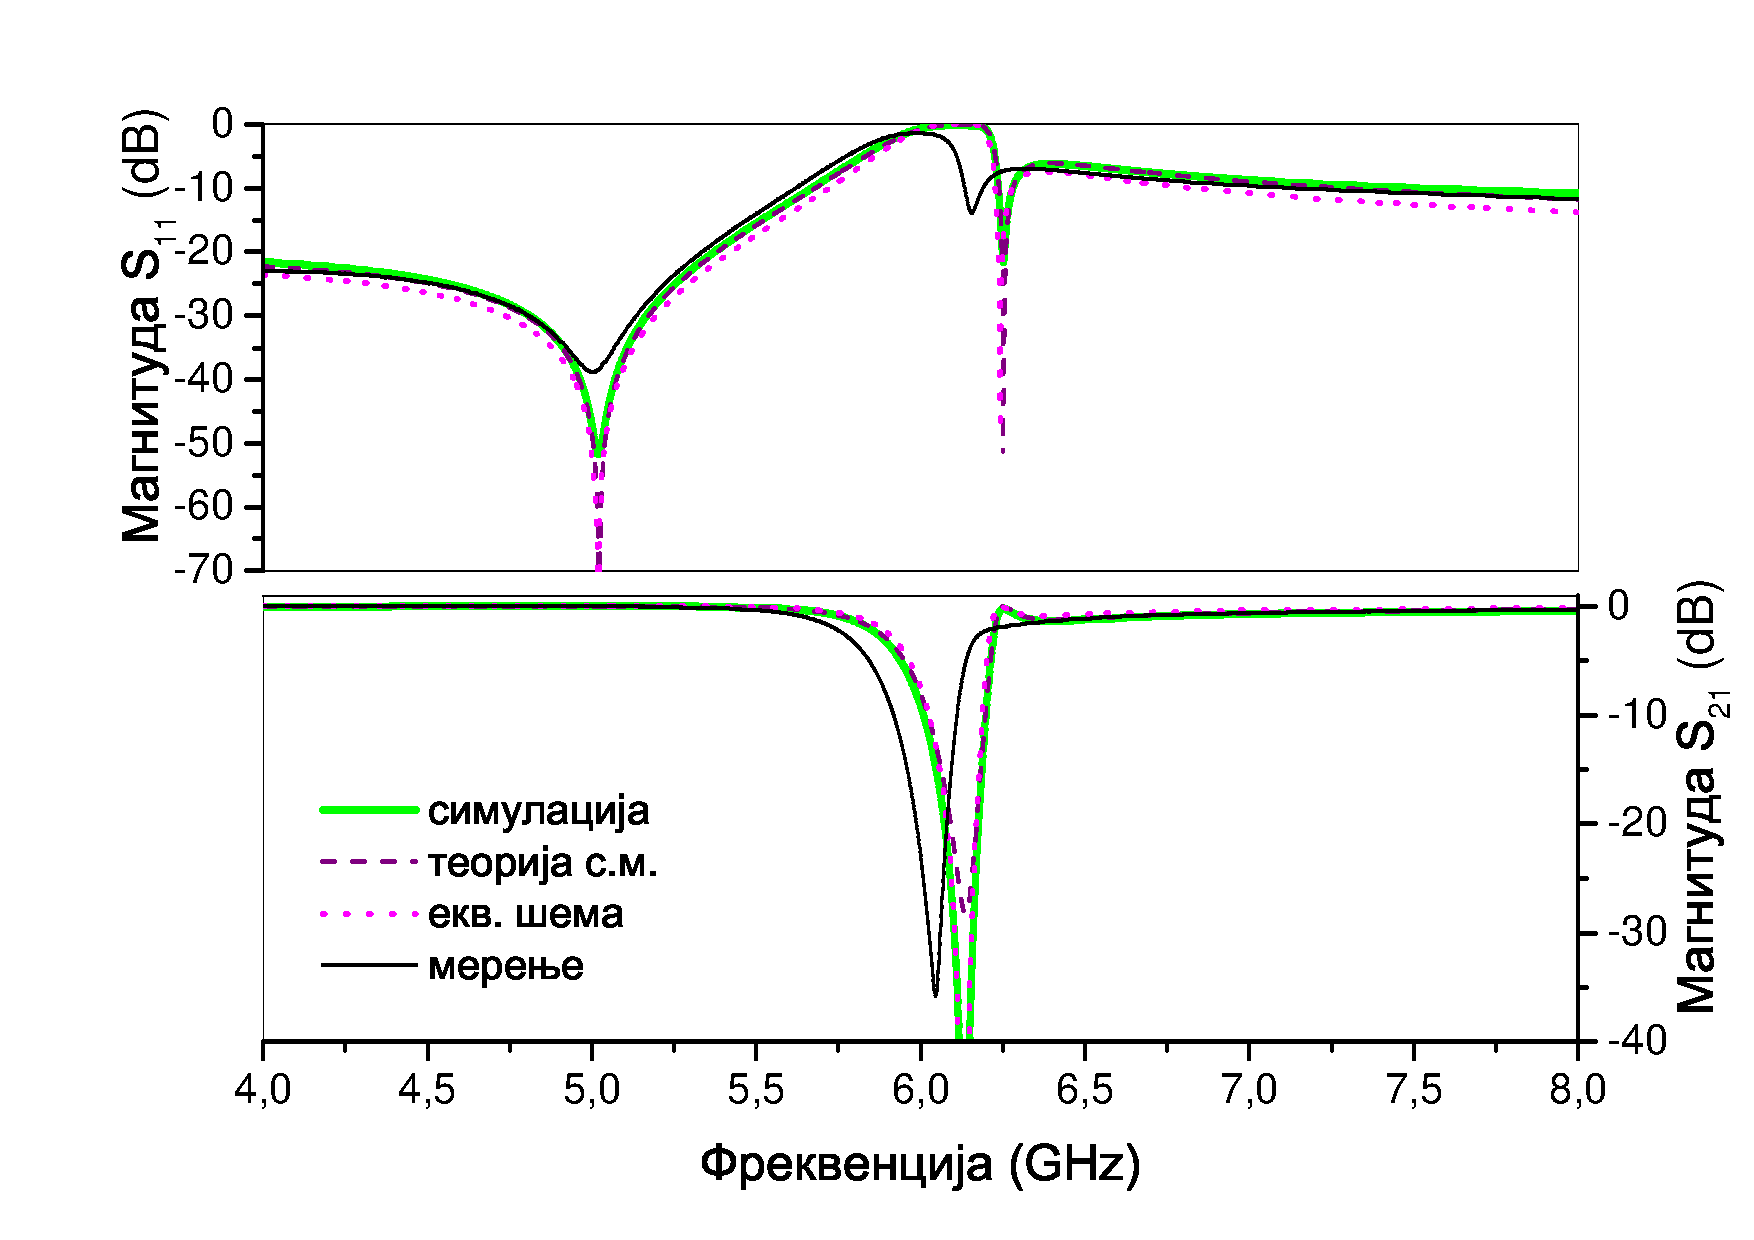
\includegraphics[width=0.5\textwidth]{sl_tsm/pod180/c_mag.pdf}}\\
\subfloat[]{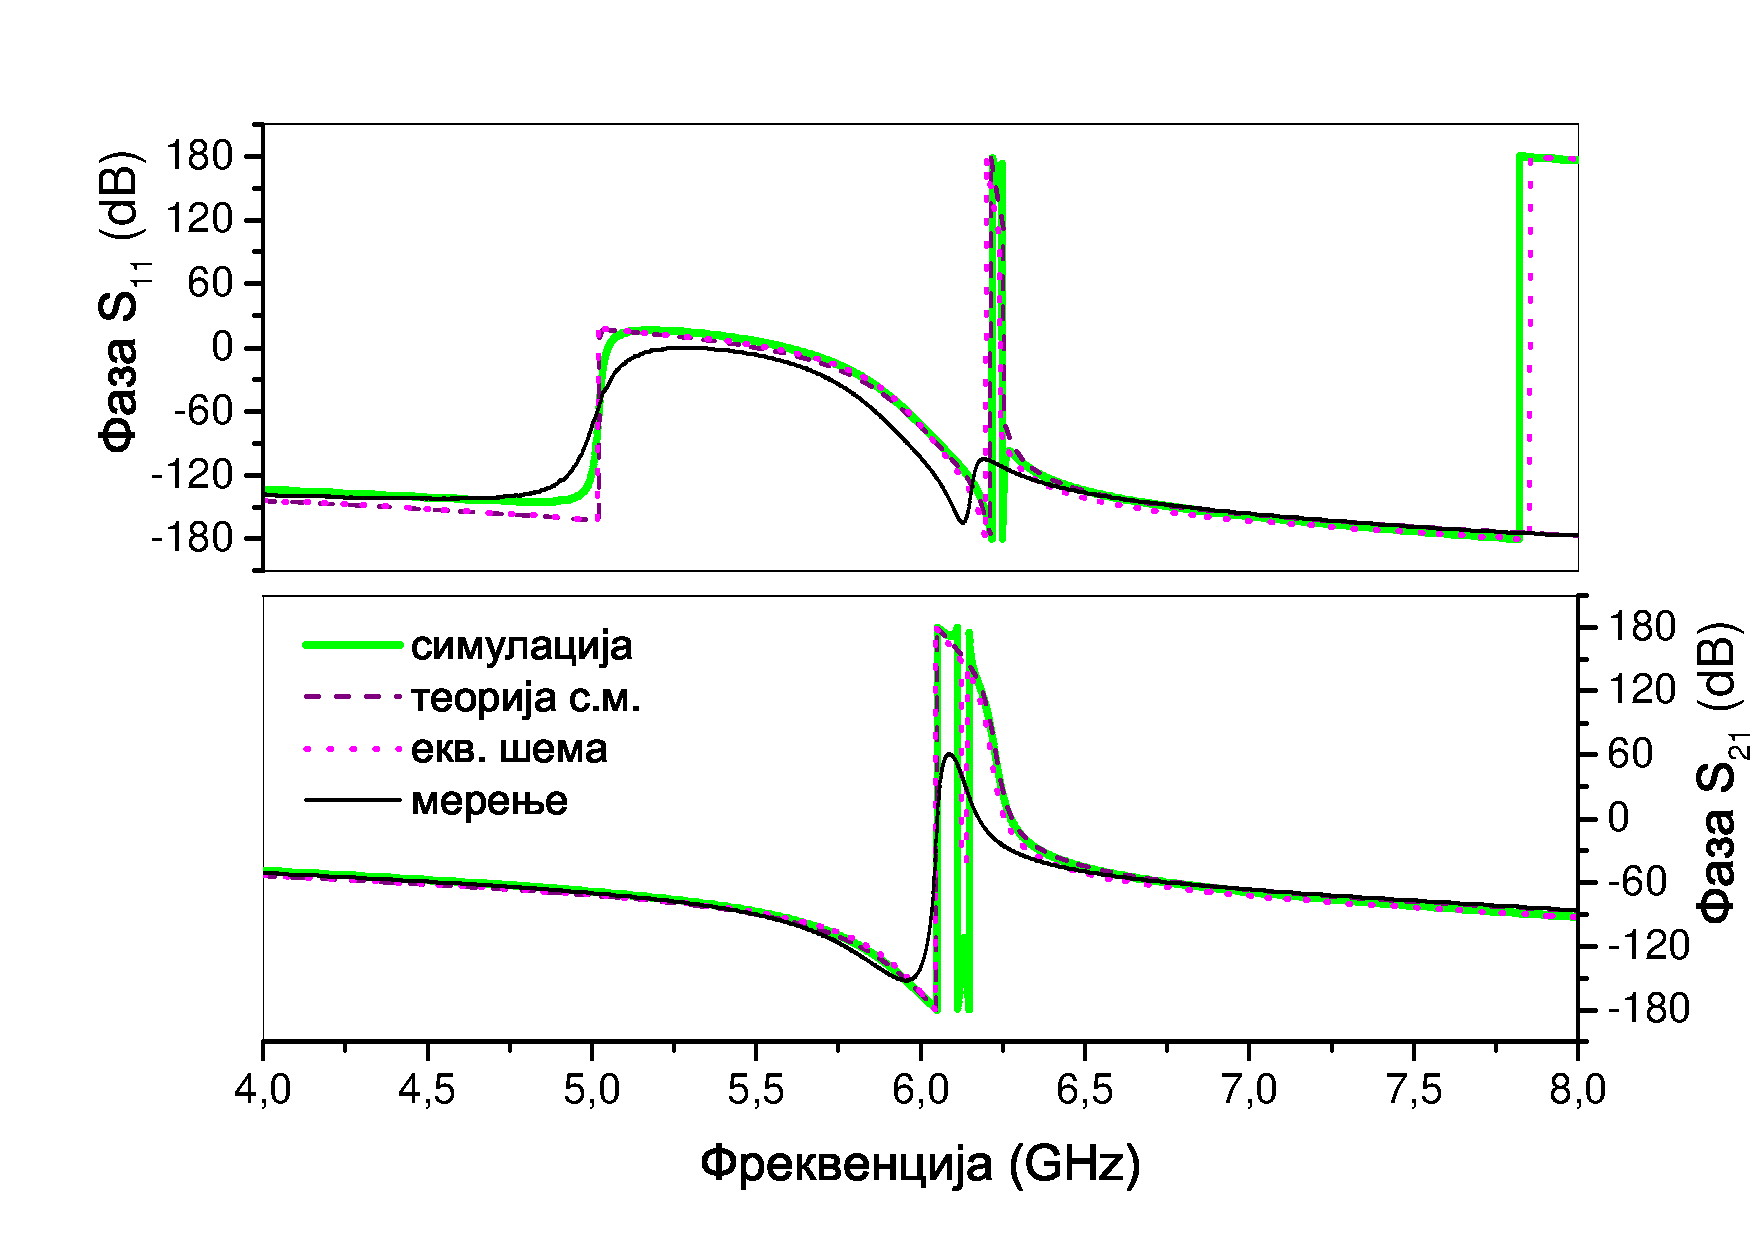
\includegraphics[width=0.5\textwidth]{sl_tsm/pod180/c_faza.pdf}}
\caption{Магнитуда и фаза $S$-параметара за модел са сл.~\ref{tsm:sl1:pod180}}
\label{tsm:rez:pod180}
\end{figure}
\begin{figure}[!t]
\centering
\subfloat[]{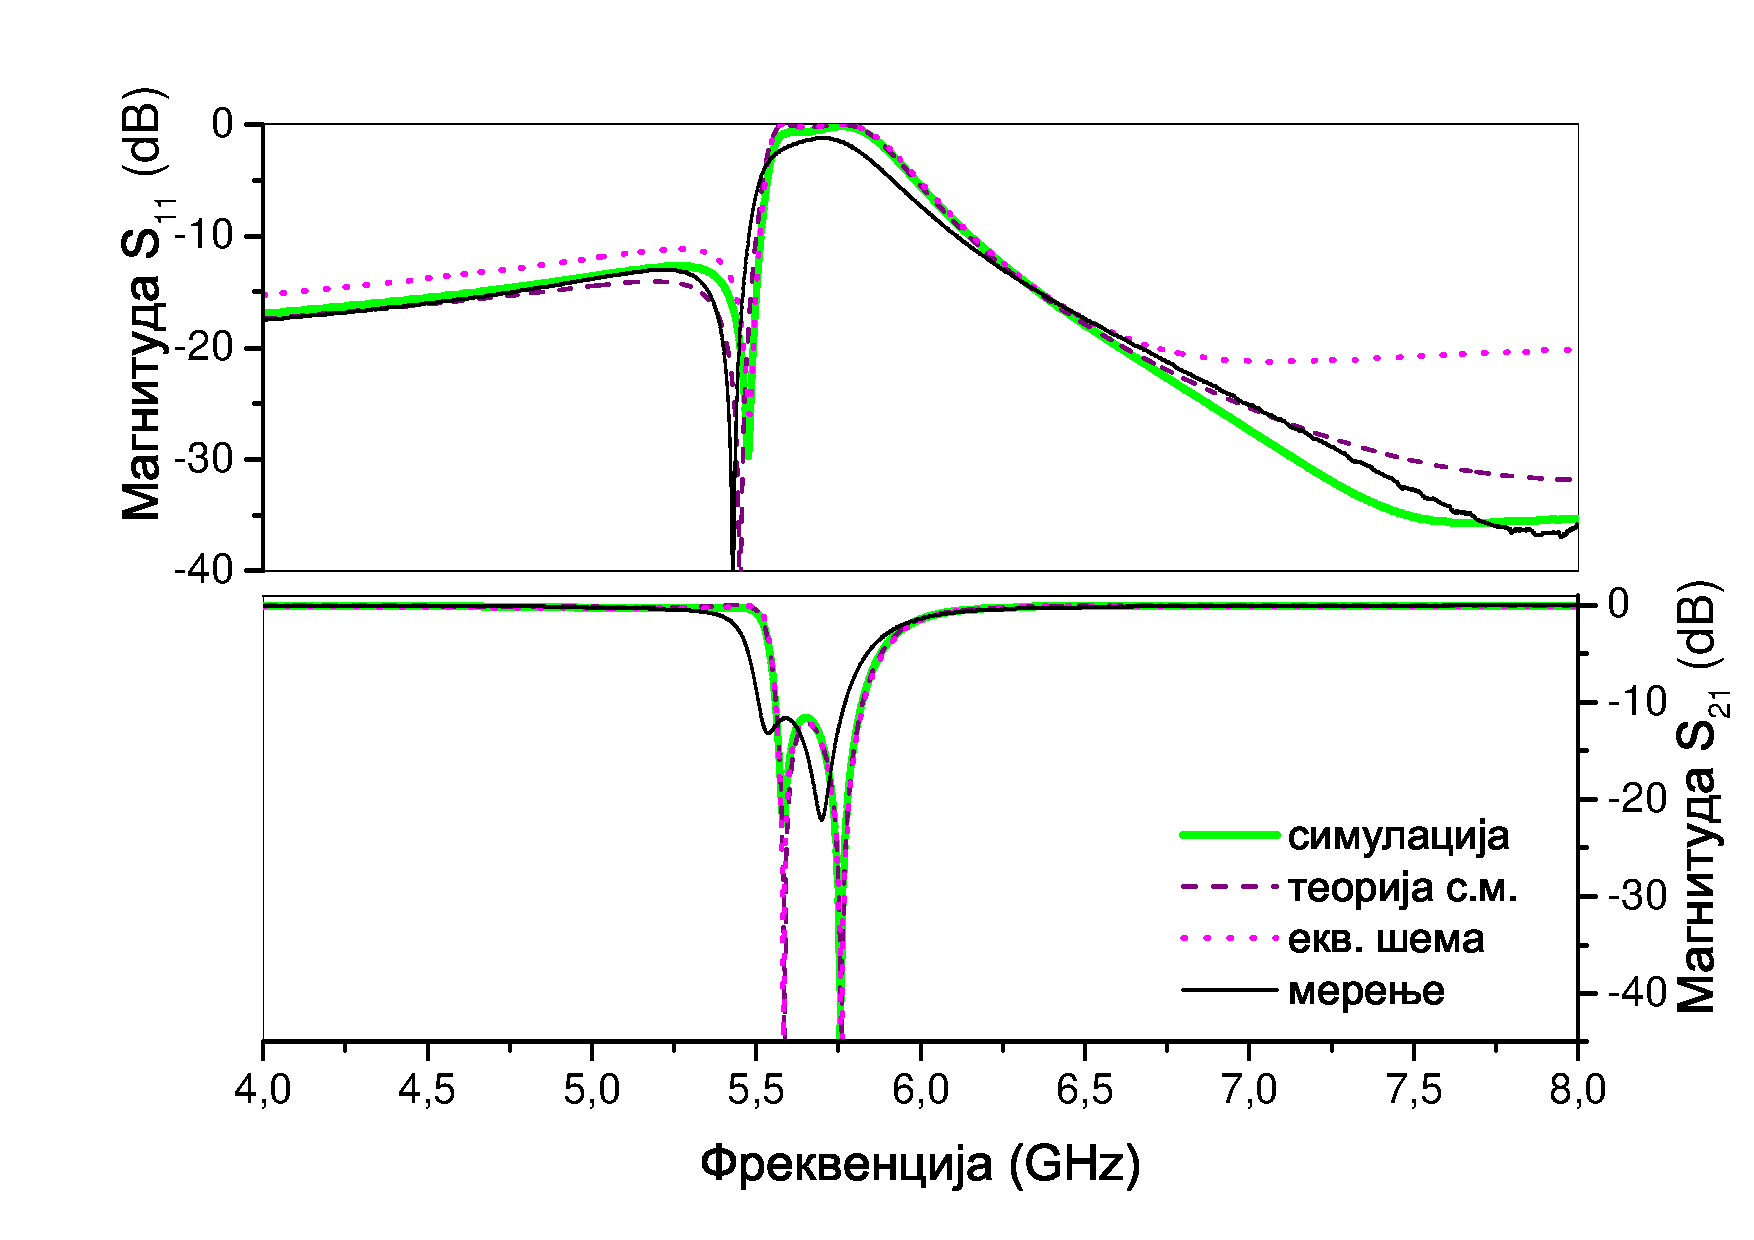
\includegraphics[width=0.5\textwidth]{sl_tsm/pod90bg/c_mag.pdf}}\\
\subfloat[]{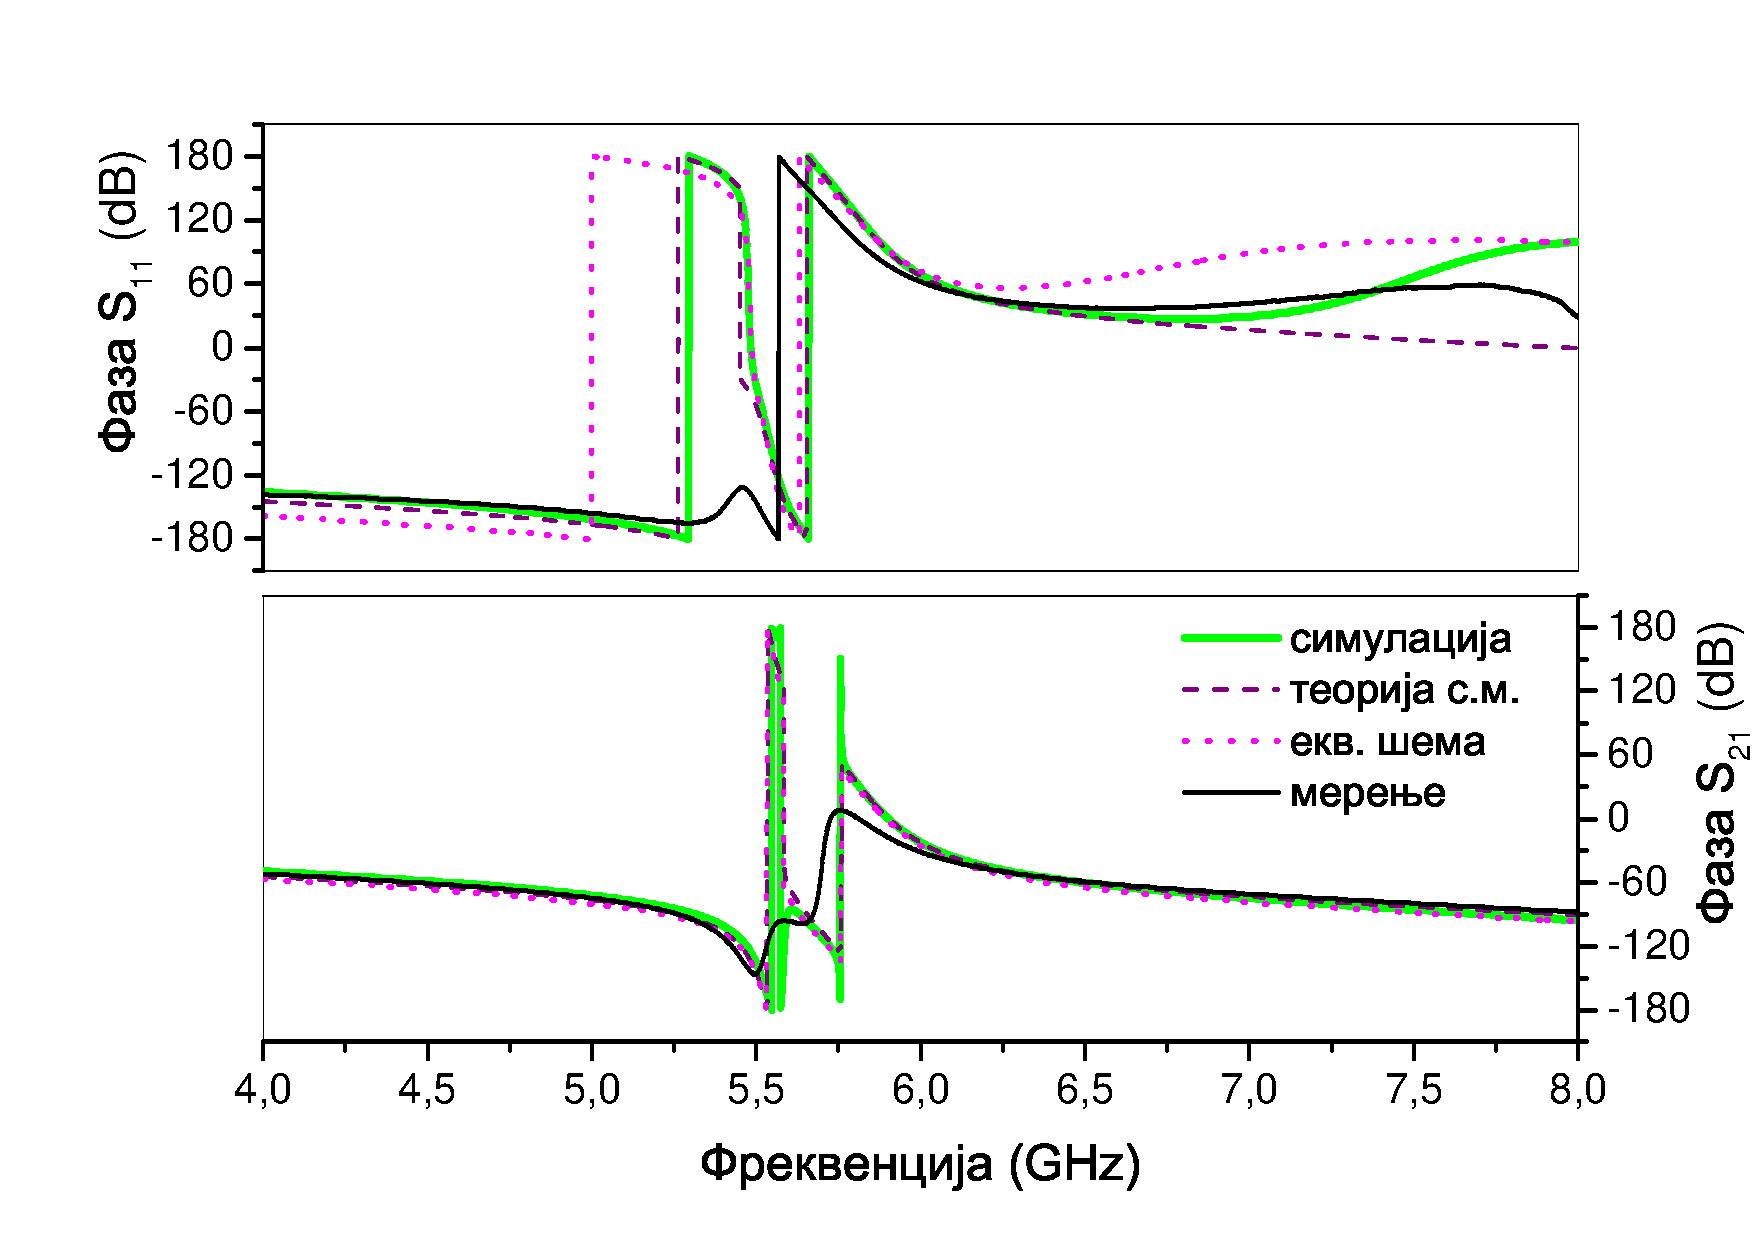
\includegraphics[width=0.5\textwidth]{sl_tsm/pod90bg/c_faza.pdf}}
\caption{Магнитуда и фаза $S$-параметара за модел са сл.~\ref{tsm:sl1:pod90bg}}
\label{tsm:rez:pod90bg}
\end{figure}
\begin{figure}[!t]
\centering
\subfloat[]{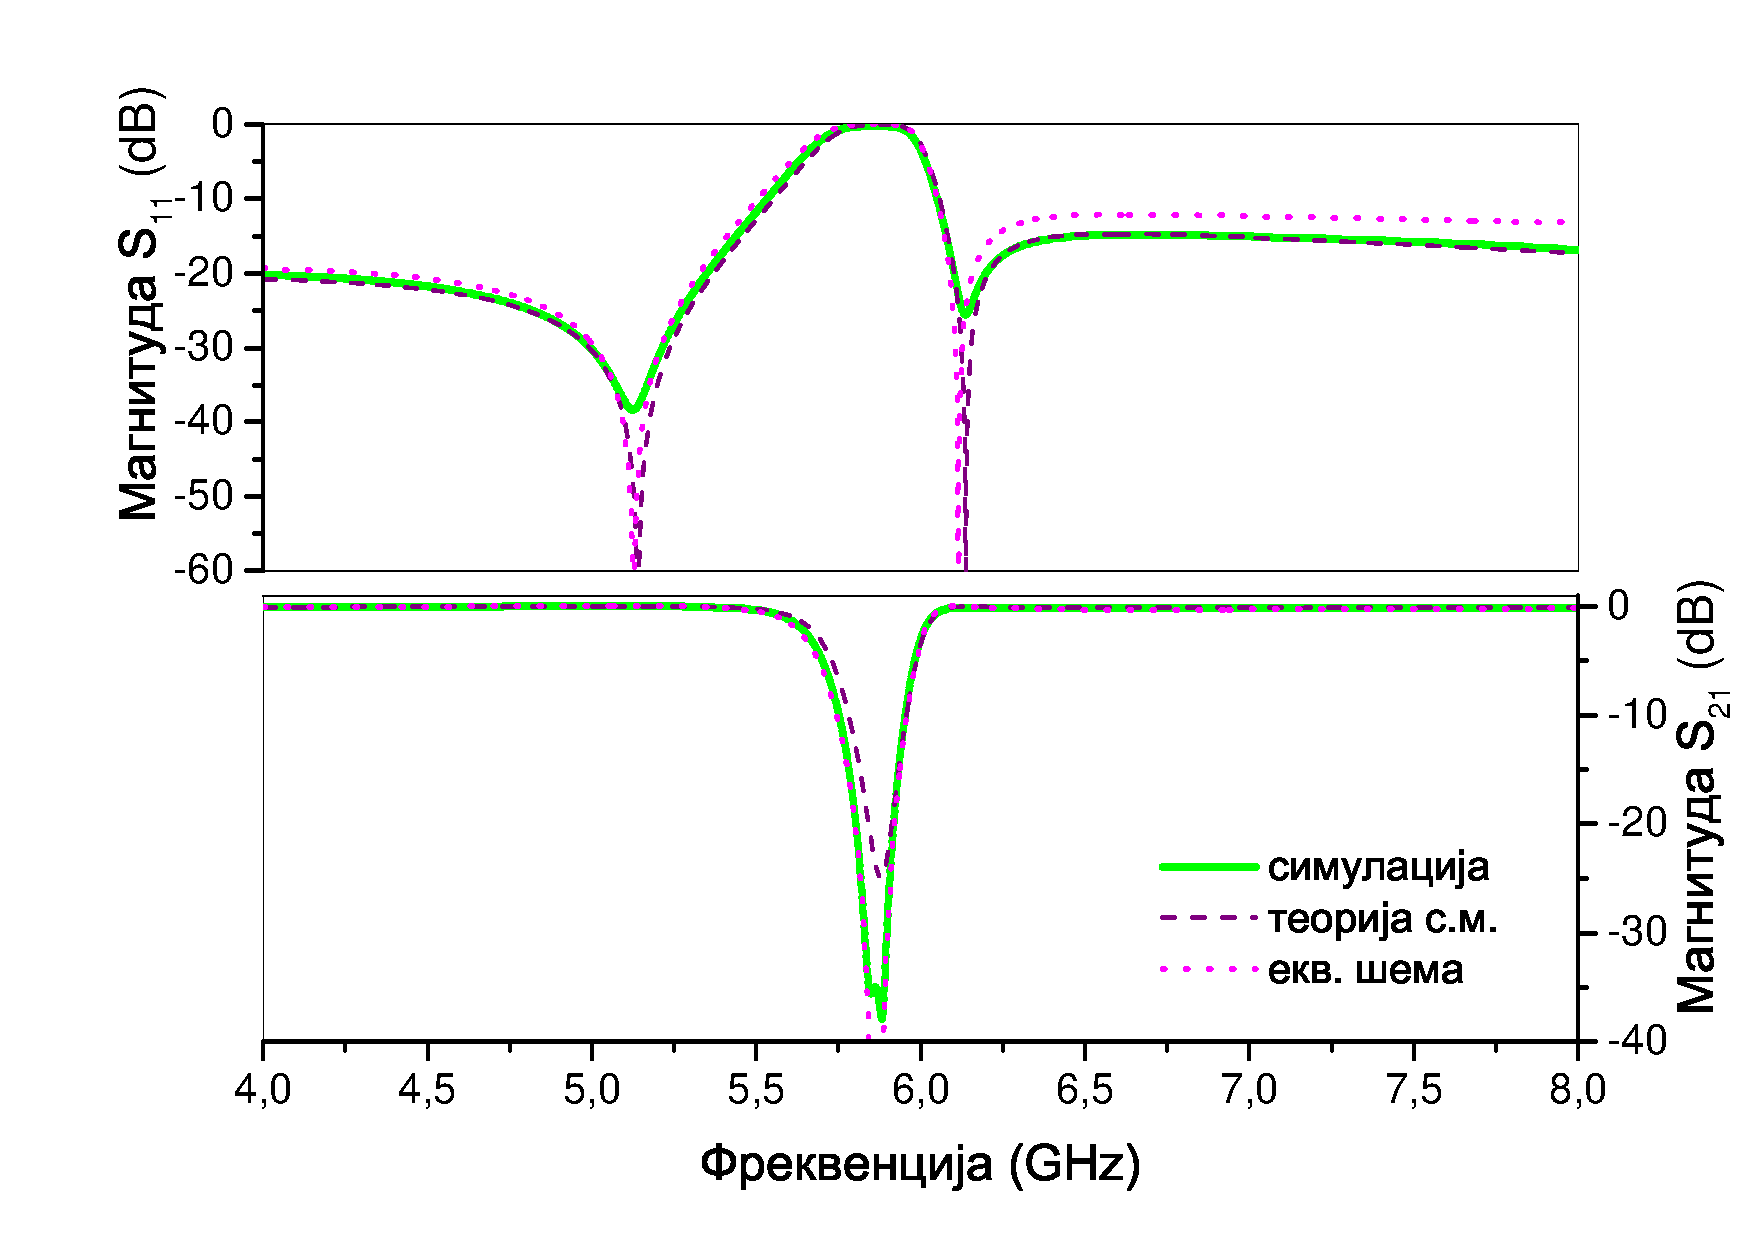
\includegraphics[width=0.5\textwidth]{sl_tsm/pod90dv/c_mag.pdf}}\\
\subfloat[]{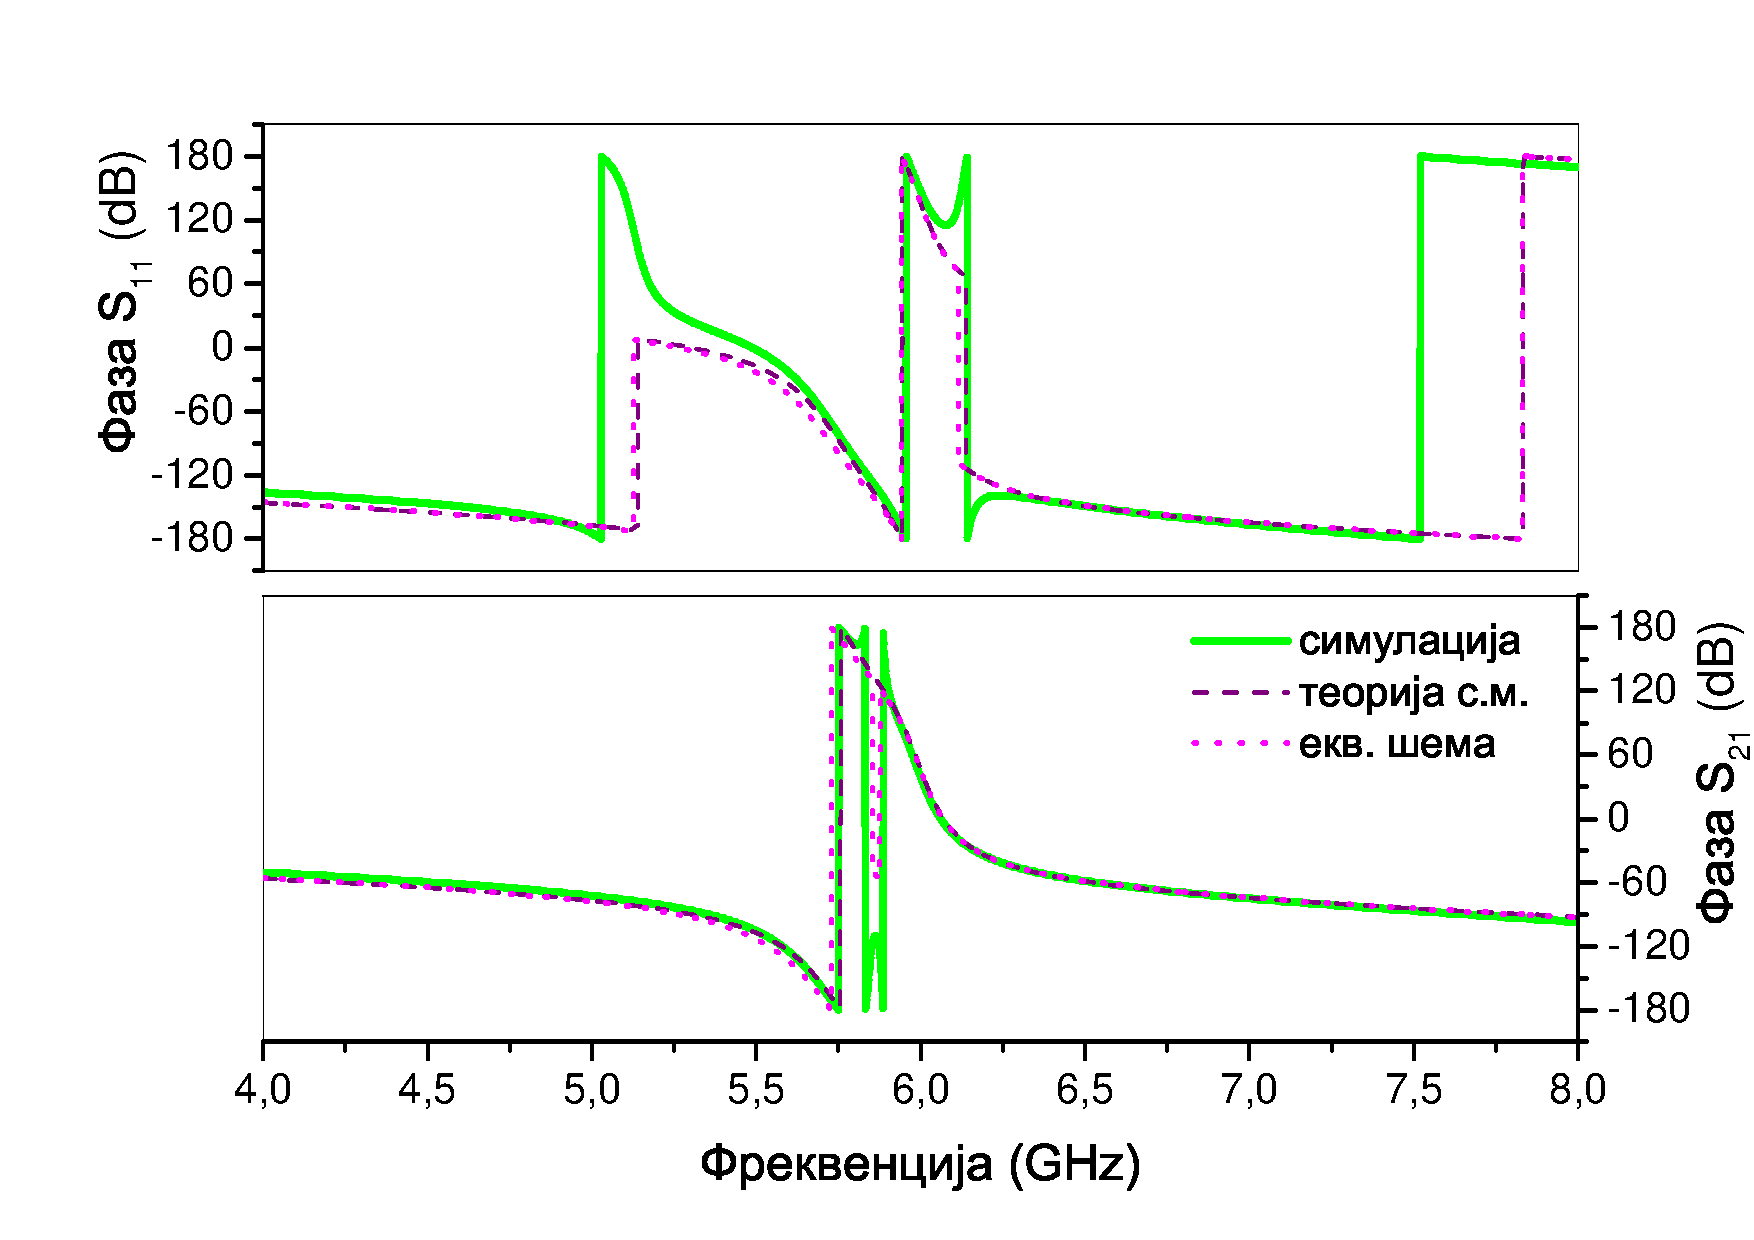
\includegraphics[width=0.5\textwidth]{sl_tsm/pod90dv/c_faza.pdf}}
\caption{Магнитуда и фаза $S$-параметара за модел са сл.~\ref{tsm:sl1:pod90dv}}
\label{tsm:rez:pod90dv}
\end{figure}
\begin{figure}[!t]
\centering
\subfloat[]{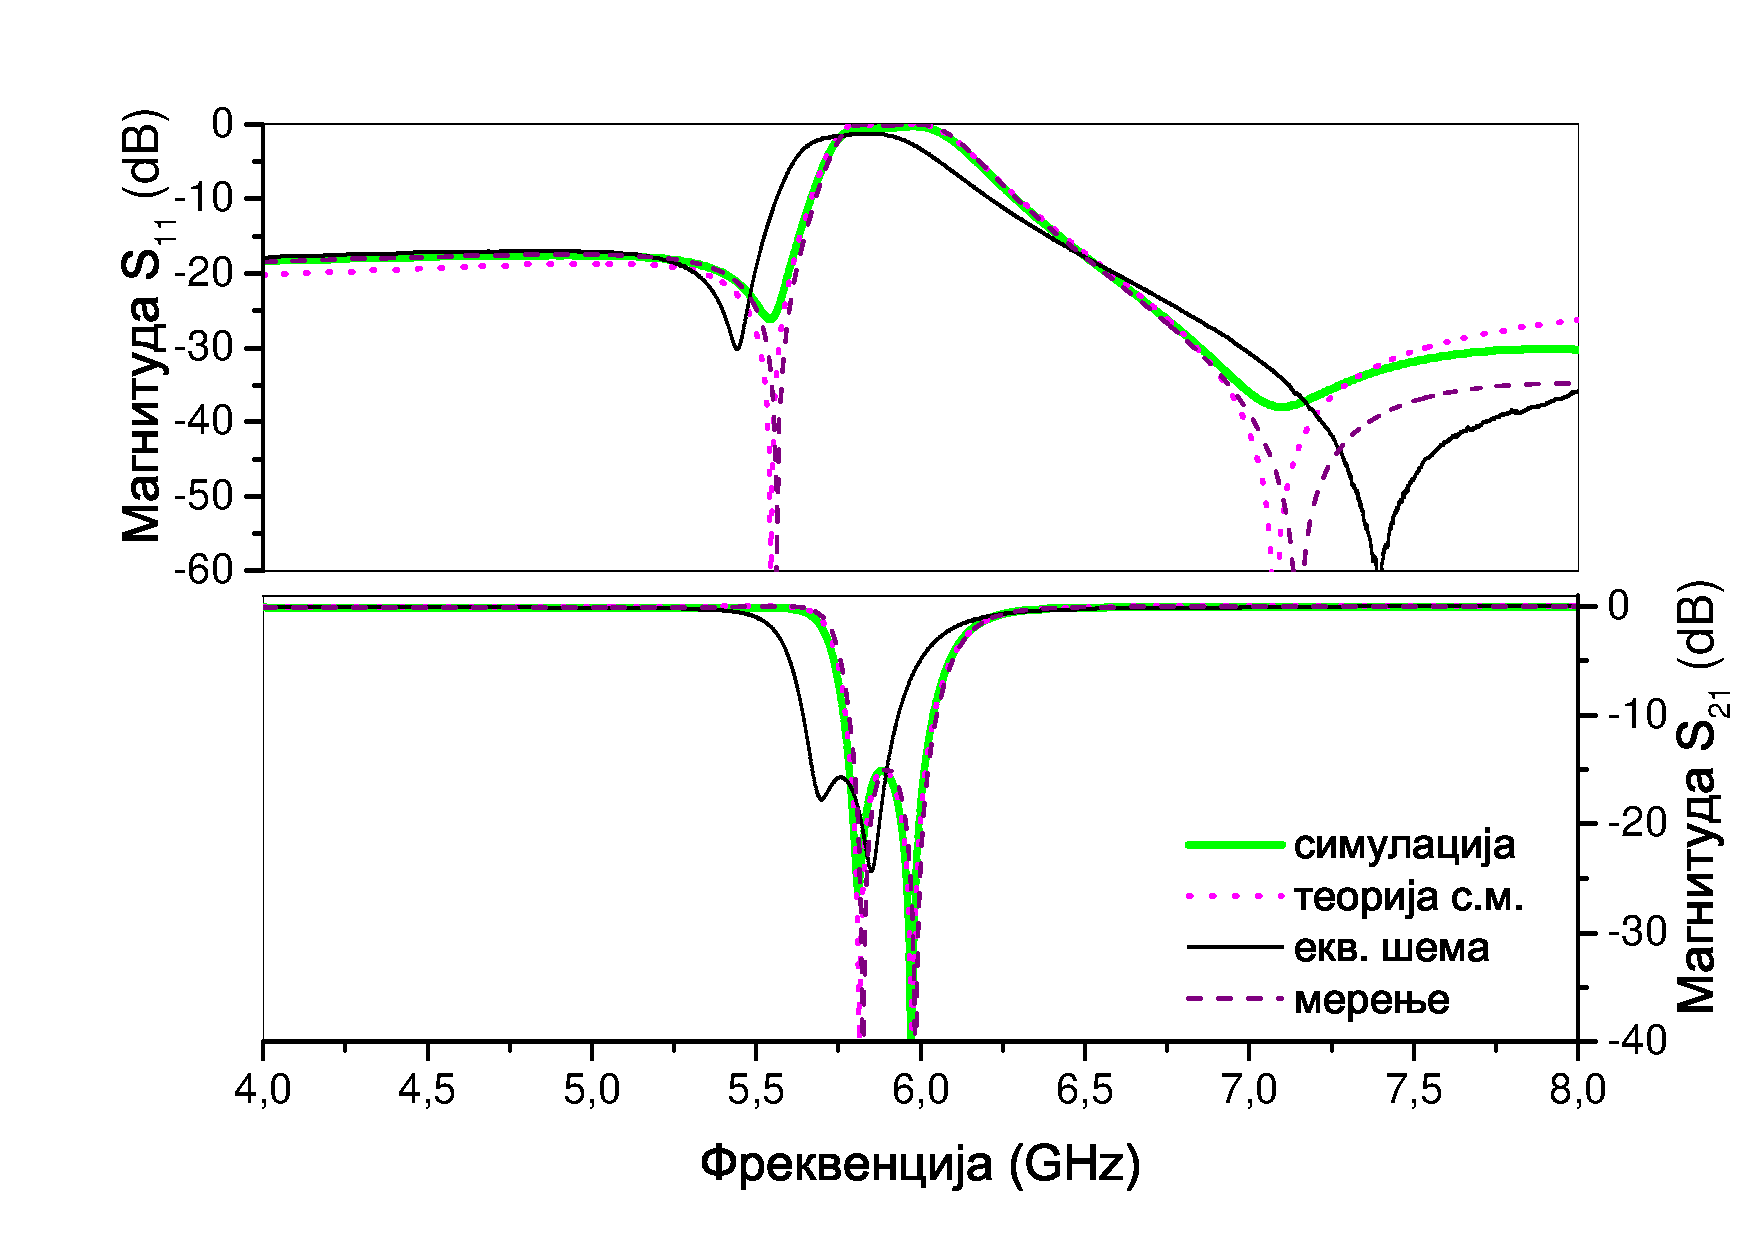
\includegraphics[width=0.5\textwidth]{sl_tsm/pod90sr/c_mag.pdf}}\\
\subfloat[]{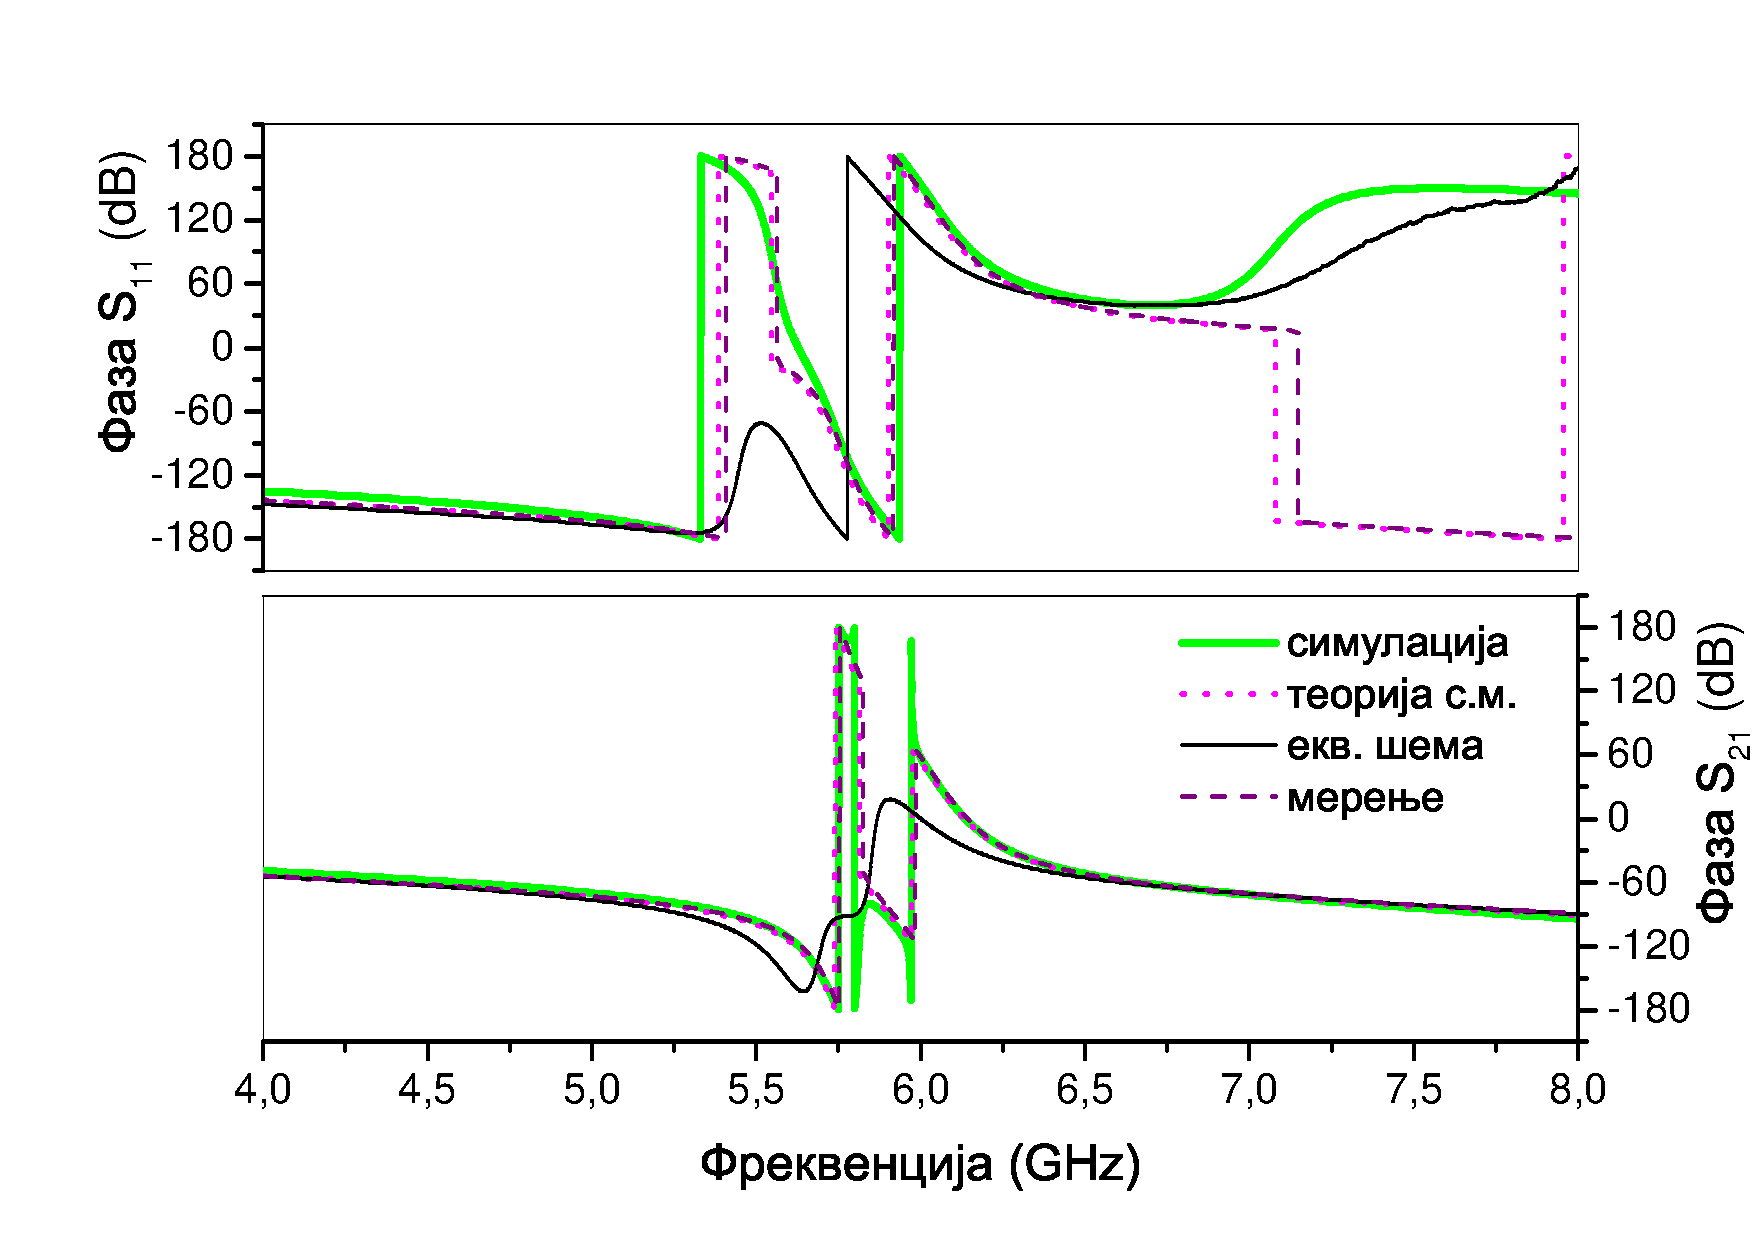
\includegraphics[width=0.5\textwidth]{sl_tsm/pod90sr/c_faza.pdf}}
\caption{Магнитуда и фаза $S$-параметара за модел са сл.~\ref{tsm:sl1:pod90sr}}
\label{tsm:rez:pod90sr}
\end{figure}
\begin{figure}[!t]
\centering
\subfloat[]{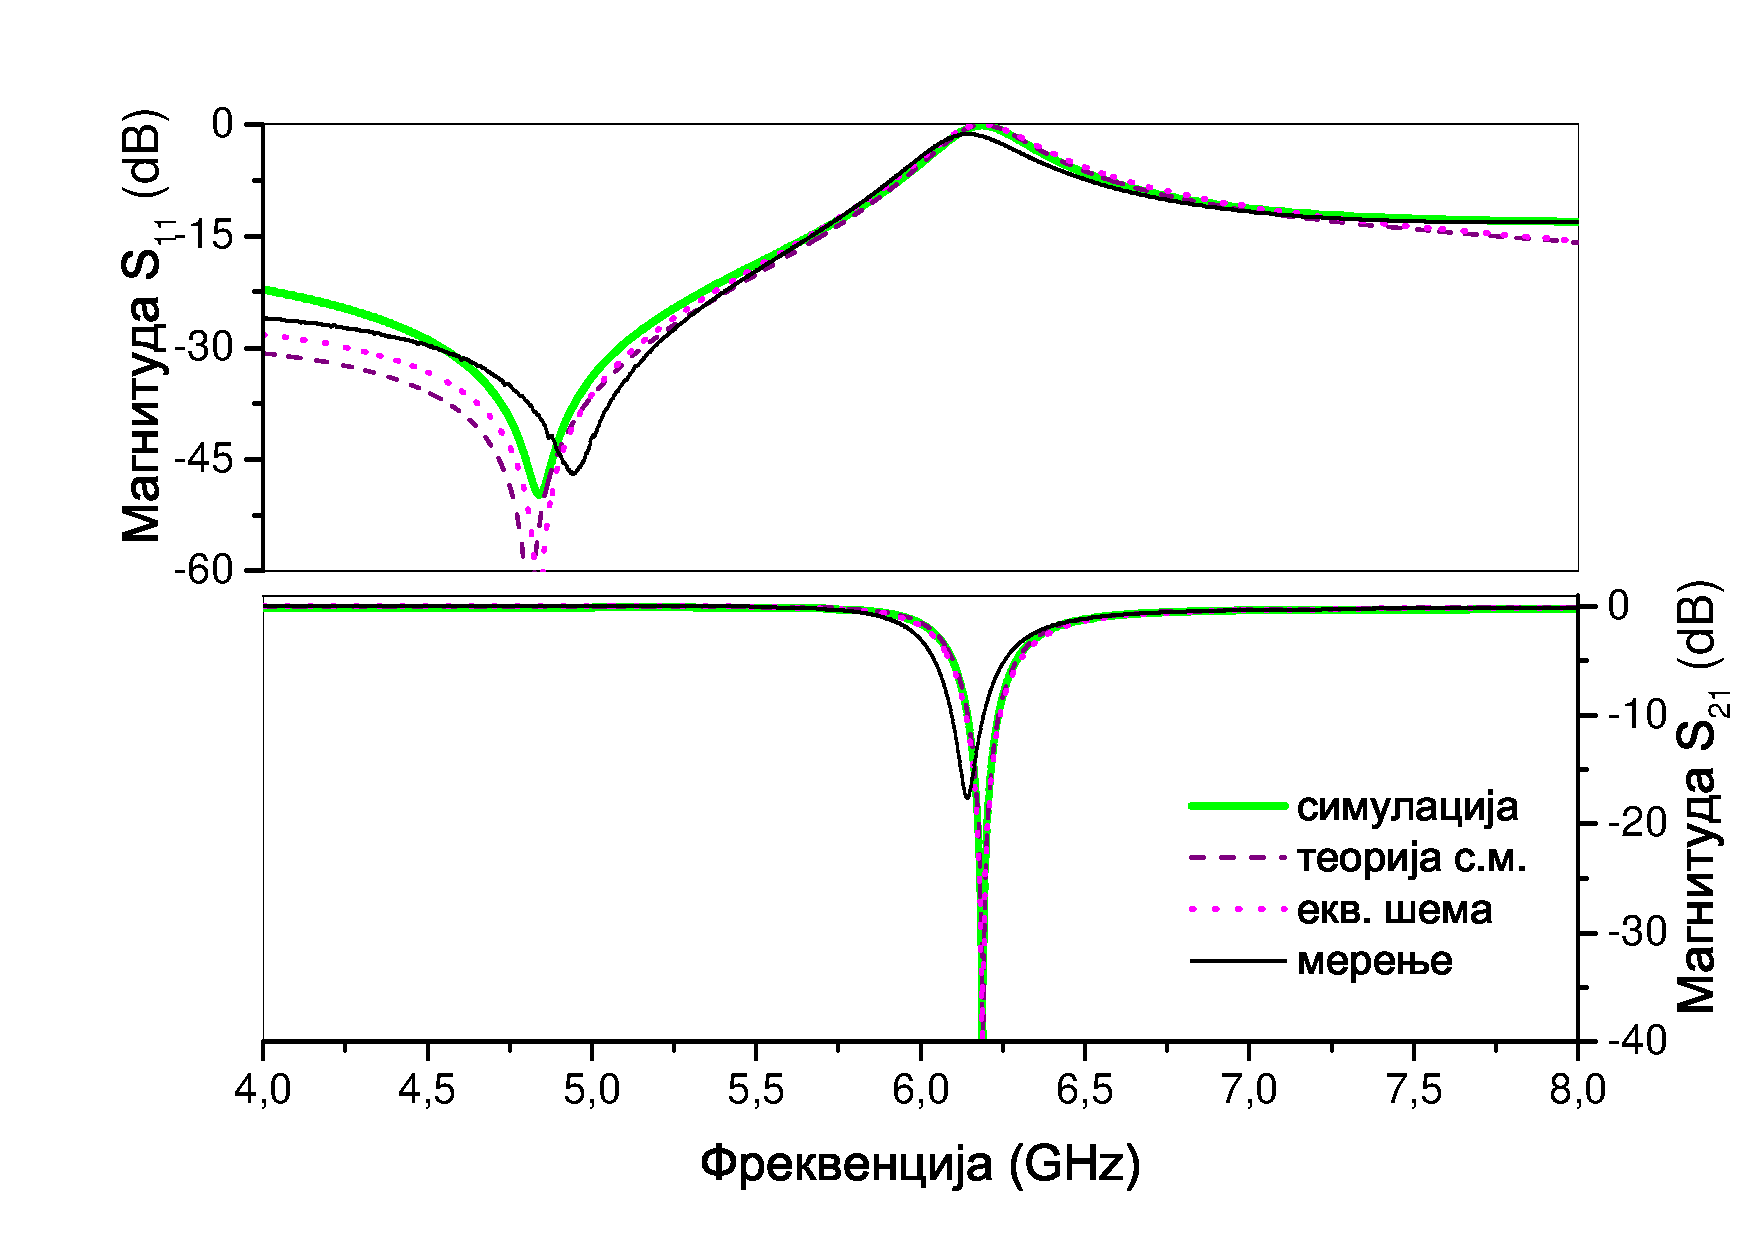
\includegraphics[width=0.5\textwidth]{sl_tsm/pod180sim/c_mag.pdf}}\\
\subfloat[]{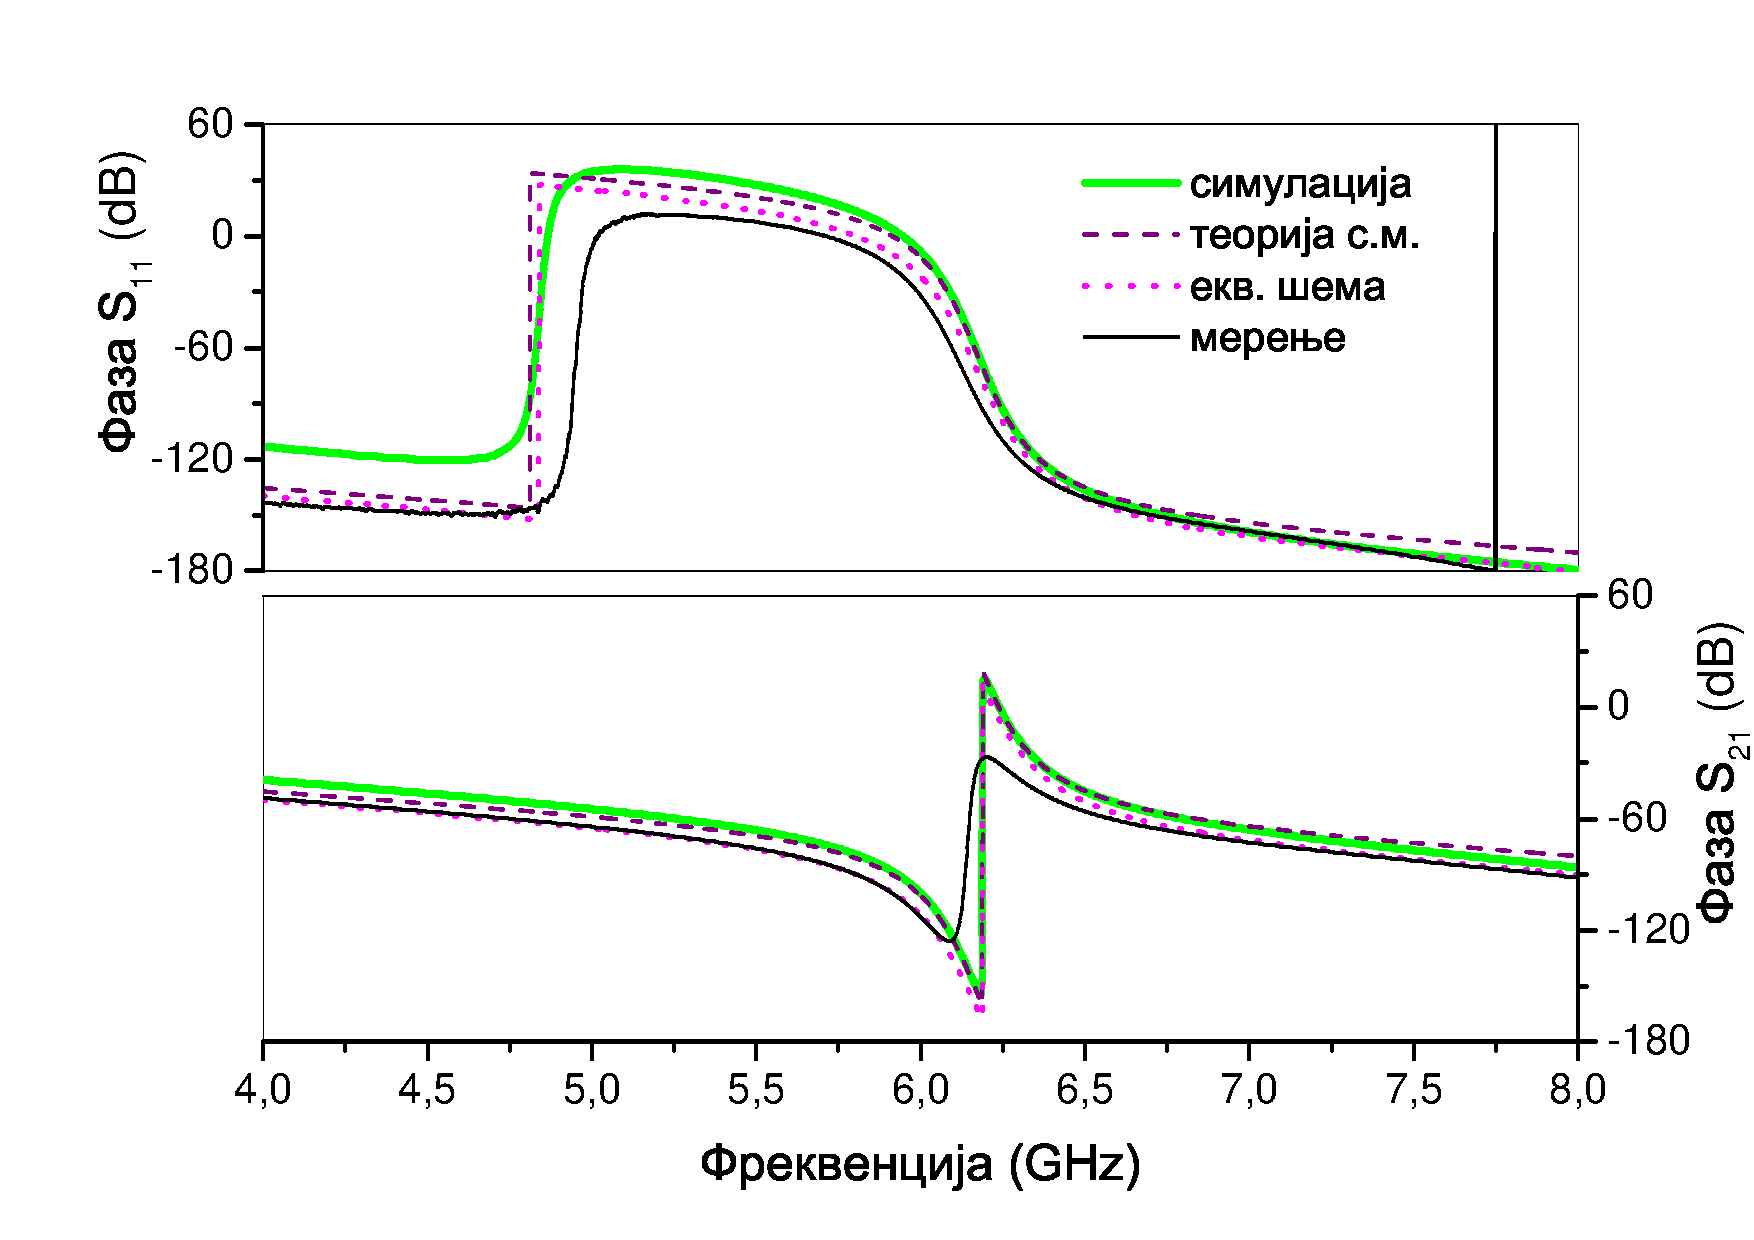
\includegraphics[width=0.5\textwidth]{sl_tsm/pod180sim/c_faza.pdf}}
\caption{Магнитуда и фаза $S$-параметара за симетрични модел. Измерени, симулирани и резултати еквивалентне шеме су преузети са сл.~12 из \cite{radoman}, а константе за ТСМ износе $L=\SI{1.23}{\nano\henry}$, $C=\SI{0.671}{\pico\farad}$, $\omega_+ = \SI{6.17}{\giga\hertz}$ и $\gamma_+ = 8.71 \times 10^8$.}
\label{tsm:rez:pod180sim}
\end{figure}

Како резултати из претходне секције нису били у потпуности задовољавајући, у наставку ће бити приказано како се може извршити њихово побољшање. Са тим циљем, користиће се еквивалентно коло са две П-ћелије (сл.~\ref{tsm:sl:ekv2cel}), пошто је очекивано да оно даје добру апроксимацију у ширем опсегу у односу на сл.~\ref{tsm:sl3}~\cite{radoman}. Треба истаћи да оба кола имају подједнак број параметара, али топологија на сл.~\ref{tsm:sl:ekv2cel} боље одражава дистрибуирану природу вода. Параметри се одређују на исти начин као и раније ($L$, $C$ и $L_S$ на основу секције вишепроводничког вода, а оснали фитовањем кривих).

У случају ТСМ, за оређивање нерезонантних параметара $\mathbf{S}^{(0)}$ користиће се модел вода са две П-ћелије (сл.~\ref{tsm:slvod:2cel}), како би више одговарао побољшаном колу. Затим, како би се добило најбоље слагање, процедура фитовања кривих биће примењена на све параметре у ТСМ моделу ($L$, $C$ са сл.~\ref{tsm:sl:vod2cel}, и $\omega_\pm$, $\gamma_\pm$). Ово ће генерално резултовати различитим вредностима $L$ и $C$ за ТСМ и еквивалентну шему, што може изгледати чудно на први поглед; међутим, треба приметити да је нерезонантни део еквивалентног кола уствари пертурбован услед присуства резонатора, као што је констатовано у секцији~\ref{tsm:sec:eqcirc}. Очекивано је да ће овај ефекат бити израженији код побољшане шеме са две ћелије, пошто је спрега СРР-ова и вода више дистрибуирана. Због тога, независно подешавање $L$ и $C$ је неопходно како би се узео у обзир ефекат ове пертурбације у ТСМ моделу.

Нови резултати за све моделе са сл.~\ref{tsm:sl1} приказани су на сл.~\ref{tsm:rez:pod0}-\ref{tsm:rez:pod90sr}, а параметри, добијени описаном процедуром, сумирани су у табели~\ref{tsm:table_konst2}. Овај пут, веома добро поклапање је добијено, не само за $S_{21}$ већ такође и за $S_{11}$, у целом разматраном фреквенцијском опсегу. Свеукупно, ТСМ и еквивалентна шема дају подједнако добре резултате, једини изузетак је неслагање у првом минимуму $S_{11}$ на сл.~\ref{tsm:rez:pod0}. Узимајући о обзир мерења на сл.~\ref{tsm:rez:pod0}, \ref{tsm:rez:pod180}, \ref{tsm:rez:pod90bg} и \ref{tsm:rez:pod90sr}, може се видети да су резонансе шире и померене ка нижим учестаностима. Ово се приписује губицима, који нису присутни у симулацијама и аналитичким моделима. Такође се може приметити да је у неким случајевима, као на сл.~\ref{tsm:rez:pod180}, \ref{tsm:rez:pod90dv}, само једна резонанса видљива у трансмисији, зато што је разлика у фреквенцијама малa у поређењу са резонантним ширинама.

Разматрањем вредности у табели ~\ref{tsm:table_konst2}, може се закључити да се укупна јачина спреге (која се може проценити као $\gamma_+ + \gamma_-$) повећава како се процеп СРР-а удаљава од вода. Ово се може објаснити помоћу расподеле струја на прстену, која има максимум у тачки која је дијаметрално супротна процепу. Такође се може видети да фитоване вредности карактеристичне импедансе вода у ТСМ моделу (сл.~\ref{tsm:slvod:2cel}), дефинисане као $Z_C = \sqrt{L/C}$, такође варирају (последње две врсте у табели~\ref{tsm:table_konst2}). Овај ефекат може се објаснити као пертурбација услед спреге, што такође објашњава неслагања у претходној секцији, где она није узета у обзир. Последично, варијација $Z_C$ је највећа у случају са најјачом спрегом (сл.~\ref{tsm:sl1:pod180}). На крају, може се видети како спрега узрокује померање резонанси ка вишим учестаностима.

Како би се тестирала њена универзалност, ТСМ је такође примењена на симетричну структуру (сл.~3c из~\cite{radoman}). У овом случају, изрази (\ref{tsm:cm_s21})--(\ref{tsm:cm_s11}) су поједностављени, пошто је присутан само симетрични мод. Резултати су приказани на сл.~\ref{tsm:rez:pod180sim}, где се види одлично слагање и у рефлексији и у трансмисији.
\begin{table}[!t]
% increase table row spacing, adjust to taste
\renewcommand{\arraystretch}{1.5}
\caption{Добијени резултати за моделе са сл.~\ref{tsm:sl1}.}
\label{tsm:table_konst2}
\centering
\begin{tabular}{|c|c|c|c|c|c|}
\hline
сл. & \ref{tsm:sl1:pod0} & \ref{tsm:sl1:pod180} & \ref{tsm:sl1:pod90bg} & \ref{tsm:sl1:pod90dv} & \ref{tsm:sl1:pod90sr} \\
\hline
\multicolumn{6}{|c|}{\emph{Еквивалентна шема}} \\
\hline
$L\,[\si{\nano\henry}]$                                       & \num{1.48}  & \num{1.47}  & \num{1.47}   & \num{1.47}  & \num{1.47} \\
\hline
$C\,[\si{\pico\farad}]$                                       & \num{0.8}   & \num{0.84}  & \num{0.84}  & \num{0.84}   & \num{0.84} \\
\hline
$L_S\,[\si{\nano\henry}]$                                     & \num{7.97}  & \num{7.91}  & \num{7.91}   & \num{7.91}  & \num{7.91} \\
\hline
$C_S\,[\si{\pico\farad}]$                                     & \num{0.105} & \num{0.09}  & \num{0.109}  & \num{0.097} & \num{0.10} \\
\hline
$k_m$                                                         & \num{0.2}   & \num{0.29}  & \num{0.276} & \num{0.32}   & \num{0.30} \\
\hline
$k_e$                                                         & \num{0.15}  & \num{0.11} & \num{0.267} & \num{0.18}    & \num{0.24} \\
\hline
$k_{m12}$                                                     & \num{0.042} & \num{0.07}  & \num{0.086} & \num{0.095}  & \num{0.10} \\
\hline
\multicolumn{6}{|c|}{\emph{Теорија спрегнутих модова}} \\
\hline
$\omega_+\,[\si{\giga\hertz}]$                                & \num{5.67}    & \num{6.23}  &  \num{5.81}  & \num{6.00}   & \num{6.06} \\
\hline 
$\omega_-\,[\si{\giga\hertz}]$                                & \num{5.52}    & \num{6.02}  &  \num{5.54}  & \num{5.75}   & \num{5.76} \\
\hline 
$\gamma_+\,[10^8 \si[per-mode=fraction]{\radian\per\second}]$ & \num{4.25}    & \num{2.01}  &  1\num{0.8}  & \num{5.08}   & \num{9.46} \\
\hline 
$\gamma_-\,[10^8 \si[per-mode=fraction]{\radian\per\second}]$ & \num{3.44}    & \num{13.8}  &  \num{3.21}  & \num{9.57}   & \num{5.18} \\
\hline 
$L\,[\si{\nano\henry}]$                                       & \num{1.46}    & \num{1.23}  &  \num{1.44}  & \num{1.35}   & \num{1.39} \\
\hline
$C\,[\si{\pico\farad}]$                                       & \num{0.762}   & \num{0.822} & \num{0.734}  & \num{0.819}  & \num{0.749} \\
\hline
\end{tabular}
\end{table} 

\section{Закључак}
У овој глави изложене су основе теорије спрегнутих модова, и демонстрирано је како се она може применити на структуре на бази метаматеријала у микроталасном опсегу. Такође је приказано како се ТСМ може применити за добијање апроксимативних аналитичких облика параметара расејања.

Структуре које су одабране за анализу састоје се од микрострип вода спрегнутог са антисиметричним сплит ринговима, и поседују симетрију у односу на ротацију од \SI{180}{\degree} око централне тачке. За разлику од структура са раванском симетријом, генерално поседују две резонансе у трансмисионом спектру, што их чини занимљивим за практичне примене.

Паралелно са ТСМ, предложена је еквивалентна шема за ове структуре, која укључује и електричну и магнетну спрегу, као и међусобну спрегу самих прстенова. Показано је како се може искористити ротациона симетрија кола за поједностављено израчунавање параметара.

Оба приступа дају аналогне резултате у близини резонанси, док се у ширем опсегу разликују. Изведене су релације које повезују параметре оба модела. Извршена су поређења са резултатима мерења и 3Д ЕМ симулација, која су потврдила теоријске закључке. Такође је приказано како се оба модела могу побољшати тако да се добије веома добро слагање, и у трансмисији и у рефлексији, у опсегу од две октаве.

Поређење два приступа показује да је израчунавање аналитичких облика параметара једноставније помоћу ТСМ, зато што инхерентно занемарује ефекте вишег реда, који нису од примарног интереса. Због тога она представља веома погодан алат за анализу расејања у системима спрегнутих резонатора.

\end{document}
